% !TeX program = xelatex
% !TeX encoding = UTF-8
% Presentazione revisionata: Azimut · Dati direzionali
% Basata sul materiale originale fornito dall'autore e sul template M01_Pensare_con_i_dati.tex
% Compilazione: xelatex -interaction=nonstopmode M18_Azimut.tex (due passaggi)
% Diagrammi TikZ e figure statistiche vettoriali; sorgenti R e dati inclusi.
% 32 slide. Materiali del corso e impaginazione della serie planetaria.
\RequirePackage{fix-cm}
\documentclass[12pt,aspectratio=1610]{beamer}
\geometry{paperwidth=20cm,paperheight=12.5cm}
\usepackage[italian,provide=*]{babel}
\usepackage{fontspec,adjustbox,tabularx}
\IfFontExistsTF{NimbusSans-Regular.otf}{
\setsansfont{NimbusSans-Regular.otf}[BoldFont=NimbusSans-Bold.otf,ItalicFont=NimbusSans-Italic.otf,BoldItalicFont=NimbusSans-BoldItalic.otf]
\setmainfont{NimbusSans-Regular.otf}[BoldFont=NimbusSans-Bold.otf,ItalicFont=NimbusSans-Italic.otf,BoldItalicFont=NimbusSans-BoldItalic.otf]
}{
\setsansfont{TeX Gyre Heros}
\setmainfont{TeX Gyre Heros}
}
\IfFontExistsTF{DejaVu Sans Mono}{
\setmonofont{DejaVu Sans Mono}[Scale=.88]
}{\setmonofont{Latin Modern Mono}[Scale=.88]}
\usefonttheme{professionalfonts}
\usepackage{amsmath,amssymb,booktabs,array,graphicx,tikz,bookmark}
\usetikzlibrary{calc,positioning,arrows.meta}
\graphicspath{{Figure/}}
\definecolor{Paper}{HTML}{F8F6F1}
\definecolor{Ink}{HTML}{253344}
\definecolor{Navy}{HTML}{15283E}
\definecolor{Quantum}{HTML}{5146A5}
\definecolor{Classical}{HTML}{087C74}
\definecolor{Muted}{HTML}{657180}
\definecolor{Rule}{HTML}{D6DAD9}
\definecolor{Night}{HTML}{112236}
\definecolor{Lilac}{HTML}{ABB5FF}
\definecolor{Mint}{HTML}{72D8C8}
\setbeamercolor{background canvas}{bg=Paper}
\setbeamercolor{normal text}{fg=Ink}
\setbeamertemplate{navigation symbols}{}
\setbeamertemplate{headline}{}
\setbeamertemplate{footline}{}
\setbeamersize{text margin left=0pt,text margin right=0pt}
\hypersetup{colorlinks=true,linkcolor=Classical,urlcolor=Classical,pdfpagemode=UseOutlines,pdfstartview=Fit,
 pdftitle={Azimut · Dati direzionali},pdfauthor={GeoStat Lab · materiali di Marzio De Corato},
 pdfsubject={GeoStat Lab · M18}}
\bookmarksetup{open,openlevel=0,depth=2}
\newsavebox{\BodyBox}
\newsavebox{\SideBox}
\newsavebox{\RecallBox}
\newsavebox{\TitleBox}
\newcommand{\MeasureBox}[2]{\typeout{REVIEWBOX:#1:\the\wd#2:\the\ht#2:\the\dp#2}}

% Revisione completa: diagrammi TikZ, formalismo e box R.
\usepackage[most]{tcolorbox}
\usepackage{listings}
\usetikzlibrary{fit,backgrounds,matrix,decorations.pathreplacing}
\definecolor{GeoA}{HTML}{1D7890}
\definecolor{GeoB}{HTML}{C57E42}
\definecolor{GeoC}{HTML}{7363AA}
\definecolor{GeoTint}{HTML}{F0F4F3}
\lstdefinestyle{GeoR}{language=R,basicstyle=\ttfamily\fontsize{9.2}{12.2}\selectfont,
 keywordstyle=\color{Quantum}\bfseries,commentstyle=\color{Classical},stringstyle=\color{GeoB},
 numbers=left,numberstyle=\tiny\color{Muted},numbersep=4pt,showstringspaces=false,
 columns=fullflexible,keepspaces=true,breaklines=true,xleftmargin=1.15em,
 frame=none,aboveskip=0pt,belowskip=0pt,tabsize=2}
\newsavebox{\PilotLeftBox}
\newsavebox{\PilotRightBox}
\newcommand{\PLabel}[1]{\par{\color{Classical}\bfseries\fontsize{9}{11}\selectfont\MakeUppercase{#1}}\par\vspace{1.8mm}}
\newcommand{\PBody}[1]{\par{\fontsize{11.3}{14.8}\selectfont #1\par}}
\newcommand{\PSmall}[1]{\par{\fontsize{9.8}{13.1}\selectfont #1\par}}
\newcommand{\PCode}[2]{%
\begin{tcolorbox}[enhanced,arc=1.8mm,boxrule=.65pt,
  colback=white,colframe=Classical!75!Navy,colbacktitle=Navy,
  coltitle=white,fonttitle=\bfseries\fontsize{9.6}{12}\selectfont,
  title={#1},left=1.7mm,right=1.3mm,top=1.5mm,bottom=1.3mm,
  before skip=1mm,after skip=1mm]
\lstinputlisting[style=GeoR]{Codice/#2}
\end{tcolorbox}}
\newcommand{\PInfo}[1]{%
\begin{tcolorbox}[enhanced,arc=1.6mm,boxrule=.55pt,colback=GeoTint,
 colframe=Rule!80!Classical,left=2.3mm,right=2.3mm,top=2mm,bottom=2mm,
 before skip=1mm,after skip=1mm]
\PSmall{#1}\end{tcolorbox}}
\tikzset{
 pFlow/.style={draw=Classical!45,fill=white,rounded corners=2mm,
  line width=.7pt,align=center,minimum height=1.1cm,font=\sffamily\fontsize{10}{12}\selectfont},
 pEdge/.style={-{Latex[length=2.3mm]},draw=Classical,line width=.95pt},
 pGroup/.style={draw=Rule,fill=white,rounded corners=2mm,line width=.65pt},
 pDotA/.style={circle,fill=GeoA,inner sep=1.25pt},
 pDotB/.style={circle,fill=GeoB,inner sep=1.25pt},
 pDotC/.style={circle,fill=GeoC,inner sep=1.25pt}
}
\newcommand{\PilotChrome}[4]{%
  \node[anchor=north west,inner sep=0,text width=17.7cm] at ([xshift=.95cm,yshift=-.55cm]current page.north west) {\color{Navy}\bfseries\fontsize{20.6}{24.5}\selectfont #1};
  \node[anchor=north east,inner sep=0] at ([xshift=19.05cm,yshift=-.14cm]current page.north west) {\color{Classical}\fontsize{8}{10}\selectfont\hyperlink{slide2}{#2}};
  \draw[Classical,line width=1.2pt] ([xshift=.95cm,yshift=-1.7cm]current page.north west)--([xshift=2.35cm,yshift=-1.7cm]current page.north west);
  \draw[Rule,line width=.65pt] ([xshift=.95cm,yshift=-10.36cm]current page.north west)--([xshift=19.05cm,yshift=-10.36cm]current page.north west);
  \node[anchor=north west,inner sep=0] at ([xshift=.96cm,yshift=-10.55cm]current page.north west) {\color{Classical}\bfseries\fontsize{9.1}{12}\selectfont DA RICORDARE};
  \node[anchor=north west,inner sep=0,text width=14.3cm] at ([xshift=4.2cm,yshift=-10.53cm]current page.north west) {\color{Ink}\fontsize{10.3}{13.8}\selectfont #4};
  \draw[Rule,line width=.35pt] ([xshift=.95cm,yshift=-11.92cm]current page.north west)--([xshift=19.05cm,yshift=-11.92cm]current page.north west);
  \node[anchor=north west,inner sep=0] at ([xshift=.95cm,yshift=-12.06cm]current page.north west) {\color{Muted}\fontsize{7.7}{9.2}\selectfont Azimut · Dati direzionali};
  \node[anchor=north east,inner sep=0] at ([xshift=19.05cm,yshift=-12.06cm]current page.north west) {\color{Muted}\fontsize{7.7}{9.2}\selectfont #3/32};
}


% Stili comuni per i diagrammi scientifici della revisione completa.
\tikzset{
 pAxis/.style={-{Latex[length=2mm]},draw=Muted,line width=.65pt},
 pNote/.style={font=\sffamily\fontsize{9}{11.5}\selectfont,text=Muted,align=center},
 pLabel/.style={font=\sffamily\fontsize{10}{12.5}\selectfont,text=Ink,align=center}
}
\newsavebox{\FullWideBox}
\setlength{\emergencystretch}{1em}




\newcommand{\PLab}[2]{\par{\color{Classical}\bfseries\fontsize{9}{11}\selectfont
\href{#1}{\MakeUppercase{#2}}}\par\vspace{1.8mm}}

\definecolor{Measure}{HTML}{A05B10}\definecolor{Rose}{HTML}{9B4564}\definecolor{Wash}{HTML}{EAE7F6}\definecolor{Gold}{HTML}{EEC184}
\tikzset{arr/.style={-{Stealth[length=2mm]},line width=.8pt,draw=Classical}}
\newcommand{\Colonna}[2]{\begin{adjustbox}{max totalsize={#1}{7.95cm},valign=t}\begin{minipage}[t]{#1}\raggedright\fontsize{11.3}{14.8}\selectfont #2\end{minipage}\end{adjustbox}}
\begin{document}

\begin{frame}[plain]\hypertarget{slide1}{}\bookmark[level=0,page=1]{Azimut}
\begin{tikzpicture}[remember picture,overlay]
\fill[Night](current page.south west) rectangle(current page.north east);
\IfFileExists{Scena/copertina.jpg}{\node[inner sep=0] at(current page.center){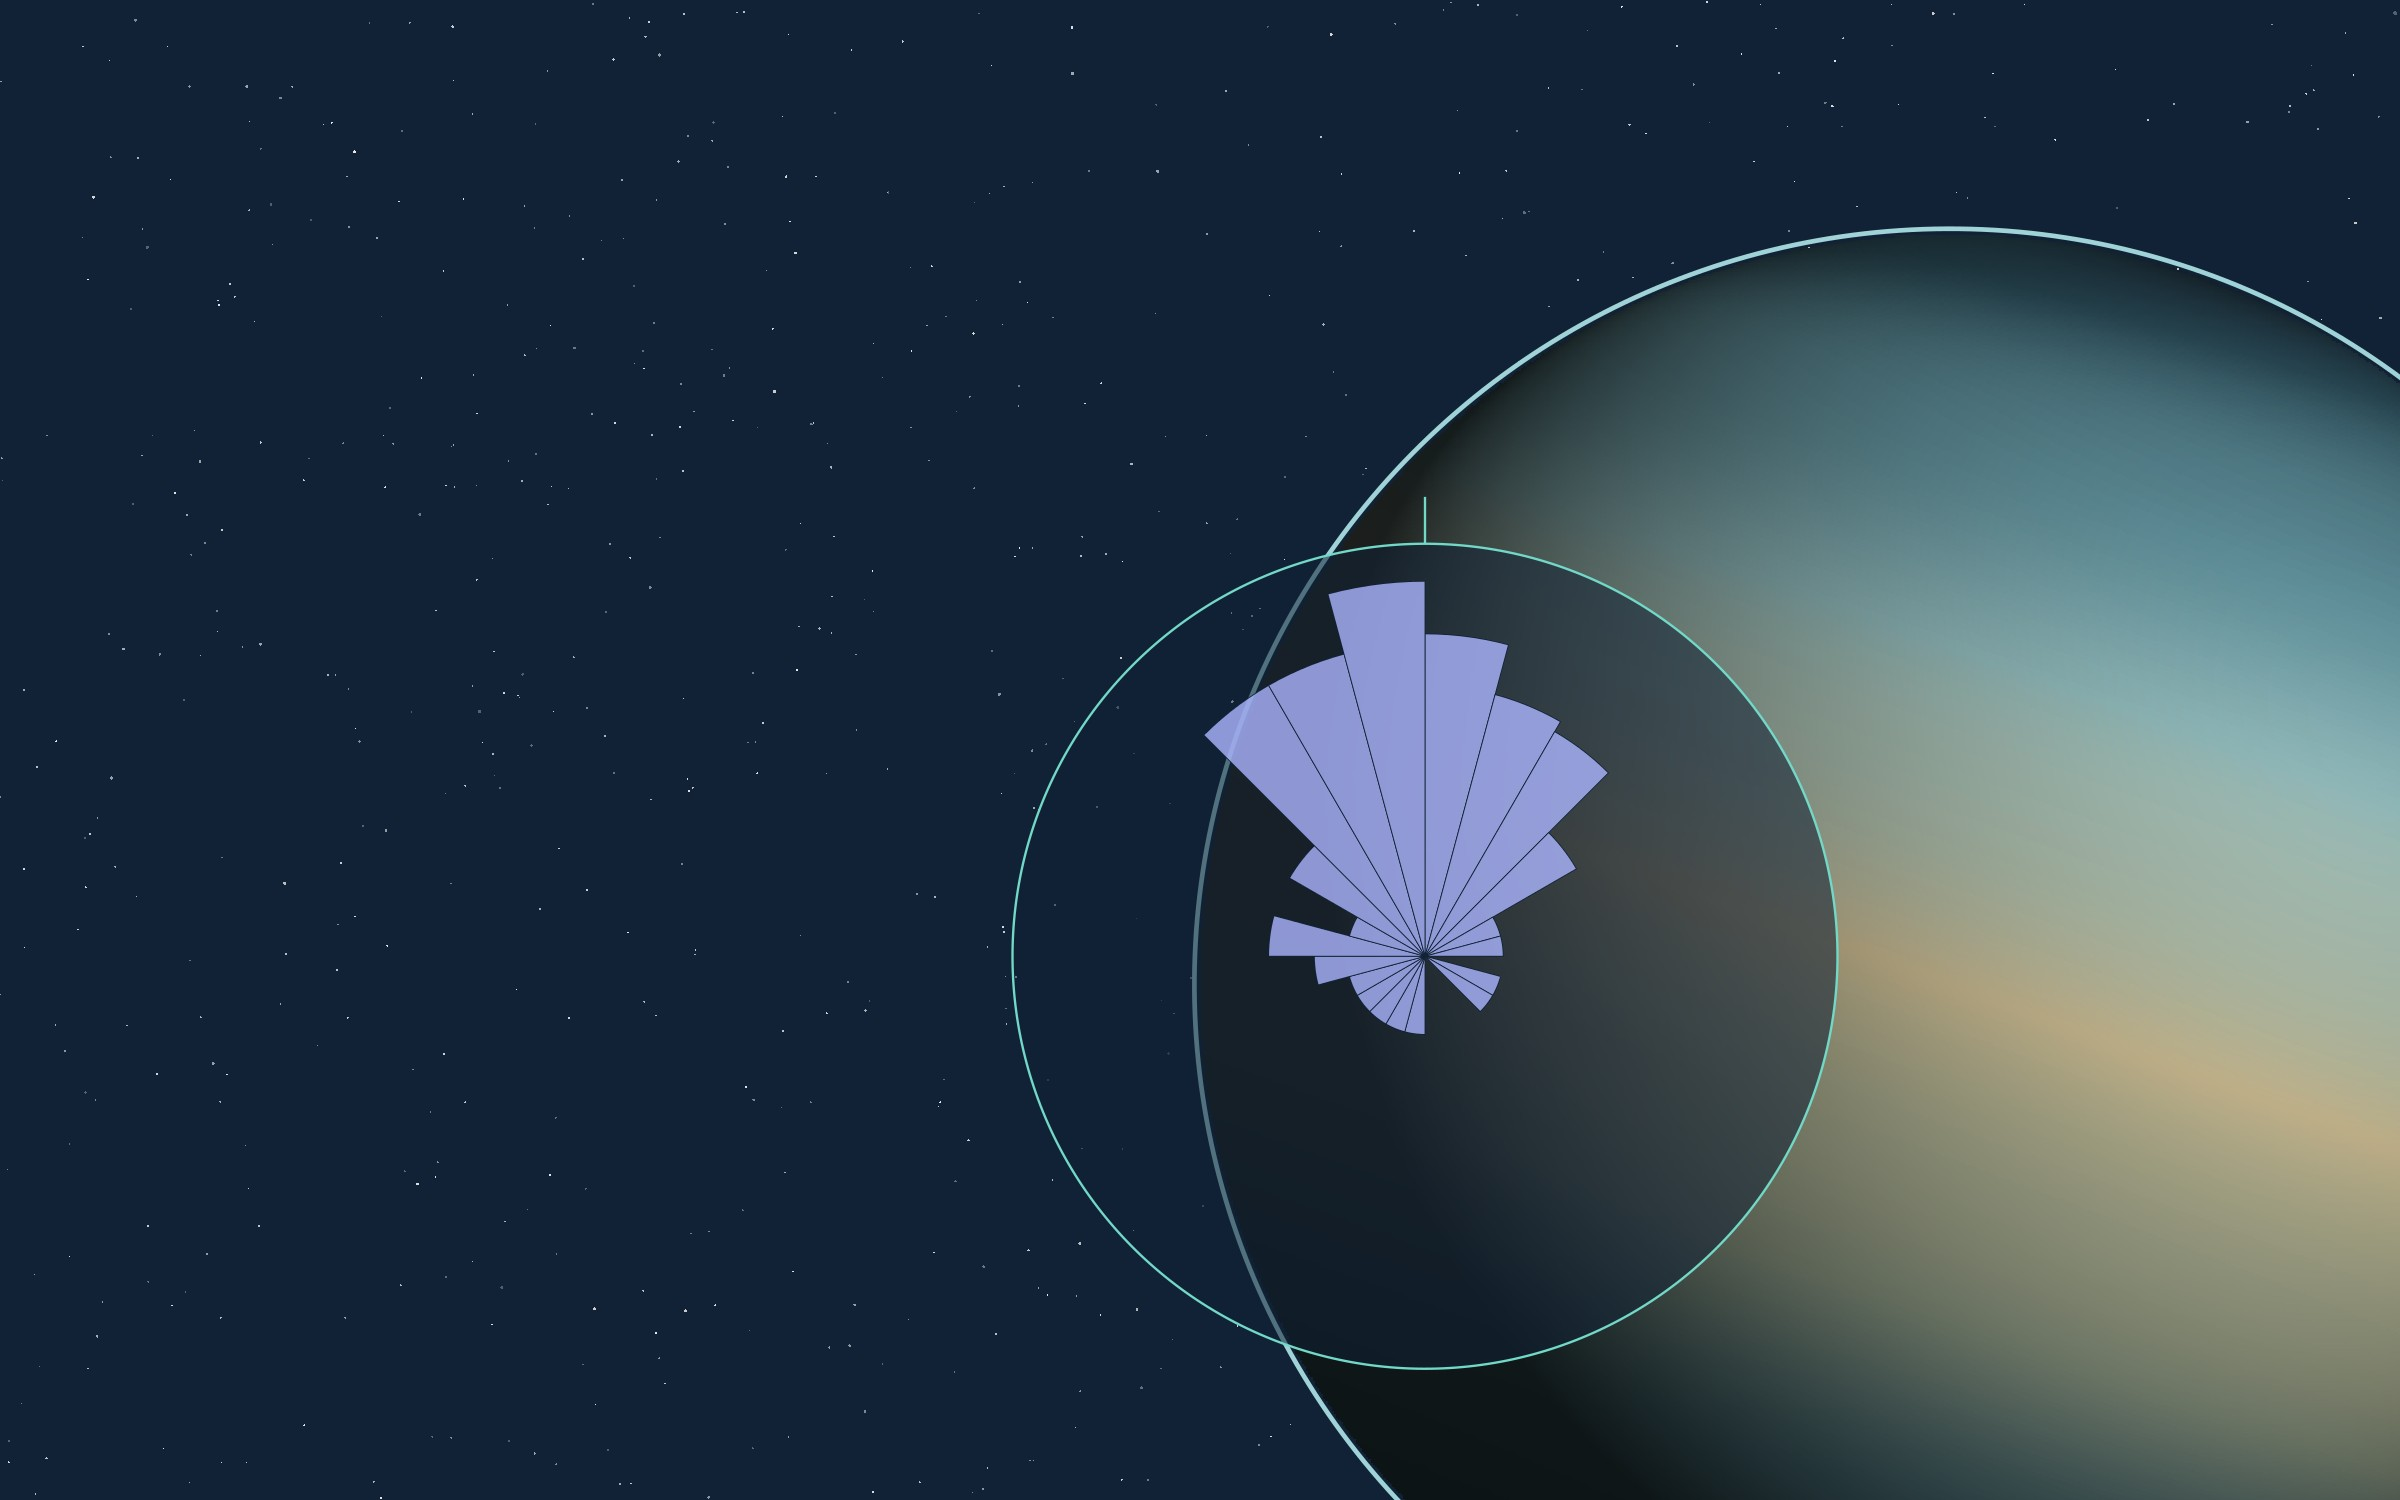
\includegraphics[width=20cm,height=12.5cm]{Scena/copertina.jpg}};}{}
\node[anchor=north west,inner sep=0] at([xshift=1.05cm,yshift=-1.10cm]current page.north west){\color{Mint}\bfseries\fontsize{23}{28}\selectfont AZIMUT};
\node[anchor=north west,inner sep=0] at([xshift=1.07cm,yshift=-2.16cm]current page.north west){\color{white}\fontsize{9}{12}\selectfont MODULO M18 · SCIENZE DELLA TERRA};
\draw[Mint,line width=1.5pt]([xshift=1.07cm,yshift=-2.78cm]current page.north west)--([xshift=2.6cm,yshift=-2.78cm]current page.north west);
\node[anchor=north west,inner sep=0] at([xshift=1.05cm,yshift=-3.35cm]current page.north west){\begin{minipage}{9.2cm}\raggedright\color{white}\bfseries\fontsize{28.5}{34.5}\selectfont Dati\\direzionali\end{minipage}};
\node[anchor=north west,inner sep=0] at([xshift=1.07cm,yshift=-7.88cm]current page.north west){\begin{minipage}{8.9cm}\raggedright\color{Lilac}\fontsize{12.2}{17}\selectfont Angoli che si chiudono su sé stessi\end{minipage}};
\node[anchor=north west,inner sep=0] at([xshift=1.07cm,yshift=-8.70cm]current page.north west){\begin{minipage}{8.9cm}\raggedright\color{white!75}\fontsize{10.3}{14.5}\selectfont Medie circolari, von Mises, assi e direzioni nello spazio\end{minipage}};
\node[anchor=north west,inner sep=0] at([xshift=1.07cm,yshift=-10.52cm]current page.north west){\color{white}\fontsize{10.5}{14}\selectfont GeoStat Lab · corso di Marzio De Corato};
\node[anchor=north west,inner sep=0] at([xshift=1.07cm,yshift=-11.17cm]current page.north west){\color{Mint}\fontsize{8.8}{11}\selectfont\href{https://creativecommons.org/licenses/by-nc-sa/4.0/}{Impaginazione da Tessera · CC BY-NC-SA 4.0}};
\end{tikzpicture}\end{frame}

\begin{frame}[plain]\hypertarget{slide2}{}
\bookmark[level=1,page=2]{Indice della presentazione}
\begin{tikzpicture}[remember picture,overlay]
\PilotChrome{Indice della presentazione}{PERCORSO}{2}{I titoli dell’indice aprono i capitoli. Il nome del capitolo in alto riporta a questa pagina.}
\node[anchor=north west,inner sep=0] at([xshift=.96cm,yshift=-2.12cm]current page.north west){\Colonna{9.40cm}{\PLabel{Capitoli}
{\fontsize{10.7}{13.5}\selectfont\hyperlink{slide4}{Angoli e direzioni medie\hfill 4}\par}\vspace{.16cm}
{\fontsize{10.7}{13.5}\selectfont\hyperlink{slide10}{La distribuzione di von Mises\hfill 10}\par}\vspace{.16cm}
{\fontsize{10.7}{13.5}\selectfont\hyperlink{slide17}{Dati assiali\hfill 17}\par}\vspace{.16cm}
{\fontsize{10.7}{13.5}\selectfont\hyperlink{slide23}{Direzioni nello spazio\hfill 23}\par}\vspace{.16cm}
}};
\node[anchor=north west,inner sep=0] at([xshift=10.85cm,yshift=-2.12cm]current page.north west){\Colonna{8.16cm}{\PLabel{Percorso di lettura}
\PBody{Centoventi azimut di paleocorrenti, centodieci direzioni di fratture, quattordici direzioni paleomagnetiche e sessanta giaciture di strati descrivono quattro modi di misurare un orientamento. Il percorso parte dalla media di angoli sul cerchio, introduce un modello e un test, tratta le linee senza verso e chiude con le direzioni nello spazio.}
\PInfo{Le pagine Scenario A e Confronto riprendono gli esperimenti nel browser. I valori di partenza del simulatore possono differire dal caso guida.}
\href{https://marzione00.github.io/Lab_Geo/\#modulo-M18}{\color{Classical}\bfseries Apri gli esperimenti di Azimut}}};
\end{tikzpicture}\end{frame}

\begin{frame}[plain]\hypertarget{slide3}{}
\bookmark[level=1,page=3]{Le paleocorrenti erano dirette verso 202,5 gradi?}
\begin{tikzpicture}[remember picture,overlay]
\PilotChrome{Le paleocorrenti erano dirette verso 202,5 gradi?}{IL CASO GUIDA}{3}{Un azimut è un punto su un cerchio: la sua scala numerica ha un inizio arbitrario.}
\node[anchor=north west,inner sep=0] at([xshift=.96cm,yshift=-2.12cm]current page.north west){\Colonna{9.40cm}{{\centering\resizebox{.97\linewidth}{!}{\begin{tikzpicture}[x=1cm,y=1cm,every node/.append style={anchor=center,inner sep=.3333em}]
\foreach \x/\n/\t/\col in {0.9/1/Medie circolari/GeoA,3.0/2/von Mises e Rayleigh/GeoC,5.1/3/Dati assiali/GeoA,7.2/4/Direzioni nello spazio/GeoB}{
 \draw[\col,fill=\col!8,rounded corners=4pt,line width=.8pt] (\x-.95,1.25) rectangle(\x+.95,3.35);
 \node[font=\bfseries\fontsize{15}{18}\selectfont,text=\col] at(\x,2.75){\n};
 \node[pNote,text width=1.75cm] at(\x,1.85){\t};}
\foreach \x in {1.85,3.95,6.05}{\draw[pEdge] (\x,2.3)--(\x+.2,2.3);}
\draw[Rule,line width=.6pt] (0,.75)--(8.15,.75);
\node[pNote] at(4.08,.35){Angoli su un cerchio: 359 e 1 grado distano due gradi.};
\end{tikzpicture}
}\par}
}};
\node[anchor=north west,inner sep=0] at([xshift=10.85cm,yshift=-2.12cm]current page.north west){\Colonna{8.16cm}{\PLabel{Il caso}
\PBody{In sei stazioni di un’unità fluviale sintetica sono stati misurati venti azimut di immersione delle lamine oblique, in gradi da nord in senso orario. La media aritmetica dei centoventi valori è 202,5 gradi. Il caso comprende anche centodieci tracce di fratture, quattordici colate con direzione di magnetizzazione nota e sessanta giaciture di strati piegati.}
\PInfo{Seguiremo i dati dalle medie circolari alla distribuzione di von Mises e al test di Rayleigh, poi agli angoli raddoppiati per le fratture e alla geometria delle direzioni nello spazio.}
}};
\end{tikzpicture}\end{frame}

\begin{frame}[plain]\hypertarget{slide4}{}
\bookmark[level=0,page=4]{Angoli e direzioni medie}
\bookmark[level=1,page=4]{Dove punta la media degli azimut?}
\begin{tikzpicture}[remember picture,overlay]
\PilotChrome{Dove punta la media degli azimut?}{ANGOLI E DIREZIONI MEDIE}{4}{La media aritmetica di angoli dipende dalla posizione dello zero della scala.}
\node[anchor=north west,inner sep=0] at([xshift=.96cm,yshift=-2.12cm]current page.north west){\Colonna{9.40cm}{\PLabel{Domanda}
\PBody{Le lamine oblique immergono per lo più fra nord-ovest e nord-est. Che cosa rappresenta la media aritmetica dei loro azimut, e quale grandezza descrive la direzione prevalente?}
\vspace{.35cm}\PLabel{Interpretazione}
\PBody{La media aritmetica vale 202,5 gradi e punta verso sud-sud-ovest, dove quasi nessuna lamina immerge. La direzione media circolare vale 352,4 gradi: le misure vicine a 350 e quelle vicine a 10 gradi sono direzioni contigue.}
}};
\node[anchor=north west,inner sep=0] at([xshift=10.85cm,yshift=-2.12cm]current page.north west){\Colonna{8.16cm}{\begin{tcolorbox}[enhanced,arc=1.7mm,boxrule=.6pt,colback=white,colframe=Classical!60!Navy,colbacktitle=Navy,coltitle=white,fonttitle=\bfseries\small,title={R · calcolo riproducibile},left=1.7mm,right=1.3mm,top=1.1mm,bottom=1.1mm,before skip=1mm,after skip=1.0mm]\lstinputlisting[style=GeoR,language=R]{Codice/capitolo-01.R}\end{tcolorbox}
\PLabel{Risultato in R}
\begin{tcolorbox}[colback=GeoTint,colframe=Rule,boxrule=.5pt,arc=1.4mm,left=2mm,right=1mm,top=1mm,bottom=1mm]{\fontsize{8.6}{11.4}\selectfont\ttfamily \mbox{aritmetica\ \ circolare}\\\mbox{\ \ \ \ \ 202.5\ \ \ \ \ \ 352.4}}\end{tcolorbox}}};
\end{tikzpicture}\end{frame}

\begin{frame}[plain]\hypertarget{slide5}{}
\bookmark[level=1,page=5]{La direzione media è quella della risultante}
\begin{tikzpicture}[remember picture,overlay]
\PilotChrome{La direzione media è quella della risultante}{ANGOLI E DIREZIONI MEDIE}{5}{Ogni misura diventa un vettore unitario; la direzione media è quella della loro somma.}
\node[anchor=north west,inner sep=0] at([xshift=.96cm,yshift=-2.12cm]current page.north west){\Colonna{9.40cm}{{\centering\resizebox{0.94\linewidth}{!}{\begin{tikzpicture}[x=1cm,y=1cm,every node/.append style={anchor=center,inner sep=.3333em}]
\draw[Rule,line width=.7pt] (0,0) circle(2.2);
\node[pNote] at(0,2.5){N};
\draw[-{Latex[length=2.4mm]},GeoA,line width=1pt] (0,0)--({2.2*sin(-10)},{2.2*cos(-10)}) node[pLabel,anchor=south east]{$350^\circ$};
\draw[-{Latex[length=2.4mm]},GeoA,line width=1pt] (0,0)--({2.2*sin(10)},{2.2*cos(10)}) node[pLabel,anchor=south west]{$10^\circ$};
\draw[-{Latex[length=2.4mm]},Classical,line width=1.6pt] (0,0)--(0,1.4);
\node[pLabel,text=Classical,anchor=west] at(.12,1.05){$\bar\theta=0^\circ$};
\draw[-{Latex[length=2.4mm]},GeoB,line width=1.1pt,dashed] (0,0)--(0,-2.2);
\node[pLabel,text=GeoB,anchor=west] at(.12,-1.6){media aritmetica $180^\circ$};
\fill[Ink] (0,0) circle(1.6pt);
\node[pNote,text width=6.4cm] at(0,-3.05){Risultante dei due vettori unitari: lunghezza $2\cos 10^\circ=1{,}97$, verso nord. Il modulo diviso per $n=2$ dà $\bar R=0{,}985$.};
\end{tikzpicture}
}\par}
\PSmall{Due misure a 350 e a 10 gradi, la loro risultante e la media aritmetica.}
}};
\node[anchor=north west,inner sep=0] at([xshift=10.85cm,yshift=-2.12cm]current page.north west){\Colonna{8.16cm}{\PBody{Ogni azimut $\theta_i$ corrisponde al vettore unitario $(\cos\theta_i,\sin\theta_i)$. La somma dei vettori ha una direzione che non dipende dallo zero della scala, e il suo modulo diviso per $n$ è la lunghezza media risultante $\bar R$: vale 1 se tutte le misure coincidono e si avvicina a 0 quando le direzioni si compensano. Joseph Curray applicò nel 1956 questa media vettoriale alle orientazioni geologiche.}
\par\smallskip{\centering\adjustbox{max width=.98\linewidth}{$\displaystyle \bar\theta=\operatorname{atan2}\big(\bar S,\bar C\big),\qquad \bar R=\sqrt{\bar C^2+\bar S^2}$}\par\smallskip}
\PSmall{$\bar C$ e $\bar S$ sono le medie di $\cos\theta_i$ e $\sin\theta_i$; la funzione atan2 restituisce l’angolo nel quadrante corretto.}
}};
\end{tikzpicture}\end{frame}

\begin{frame}[plain]\hypertarget{slide6}{}
\bookmark[level=1,page=6]{La rosa a settori di uguale area}
\begin{tikzpicture}[remember picture,overlay]
\PilotChrome{La rosa a settori di uguale area}{ANGOLI E DIREZIONI MEDIE}{6}{In una rosa il raggio di ogni settore va preso proporzionale alla radice della frequenza.}
\node[anchor=north west,inner sep=0] at([xshift=.96cm,yshift=-2.12cm]current page.north west){\Colonna{9.40cm}{{\centering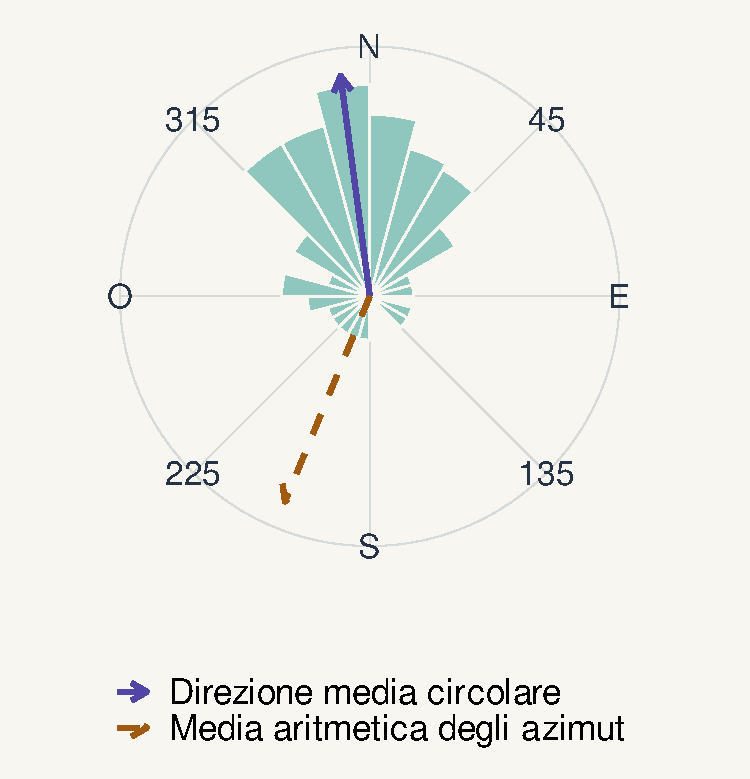
\includegraphics[width=\linewidth,height=6.3cm,keepaspectratio]{Figure/F01.pdf}\par}
\PSmall{Centoventi azimut in classi di 15 gradi; le frecce indicano la direzione media e la media aritmetica.}
}};
\node[anchor=north west,inner sep=0] at([xshift=10.85cm,yshift=-2.12cm]current page.north west){\Colonna{8.16cm}{\PBody{La rosa è l’istogramma di dati circolari. Se il raggio di un settore cresce con la frequenza, la sua area cresce con il quadrato e la classe modale appare esagerata: Wojciech Nemec lo osservò nel 1988, e David Sanderson e David Peacock hanno ripreso il problema nel 2020. Qui il raggio è proporzionale alla radice della frequenza. La lunghezza media risultante dei centoventi azimut è 0,756.}
\PSmall{Come per un istogramma, la forma della rosa dipende dall’ampiezza e dall’origine delle classi.}
}};
\end{tikzpicture}\end{frame}

\begin{frame}[plain]\hypertarget{slide7}{}
\bookmark[level=1,page=7]{Direzione, concentrazione e dispersione per stazione}
\begin{tikzpicture}[remember picture,overlay]
\PilotChrome{Direzione, concentrazione e dispersione per stazione}{ANGOLI E DIREZIONI MEDIE}{7}{La deviazione standard circolare si ricava da $\bar R$ e si esprime in gradi.}
\node[anchor=north west,inner sep=0] at([xshift=.96cm,yshift=-2.12cm]current page.north west){\Colonna{9.40cm}{\PBody{Per ogni stazione il codice calcola direzione media, lunghezza media risultante e deviazione standard circolare. Cinque stazioni hanno $\bar R$ fra 0,82 e 0,95 e direzioni fra 349 e 14 gradi. La stazione S6 ha $\bar R=0{,}31$ e una deviazione standard di 88 gradi: le sue direzioni sono molto disperse. La varianza circolare $1-\bar R$ vale 0,244 per l’insieme delle misure.}
\par\smallskip{\centering\adjustbox{max width=.98\linewidth}{$\displaystyle \sigma_c=\sqrt{-2\log\bar R}$}\par\smallskip}
}};
\node[anchor=north west,inner sep=0] at([xshift=10.85cm,yshift=-2.12cm]current page.north west){\Colonna{8.16cm}{\begin{tcolorbox}[enhanced,arc=1.7mm,boxrule=.6pt,colback=white,colframe=Classical!60!Navy,colbacktitle=Navy,coltitle=white,fonttitle=\bfseries\small,title={R · calcolo riproducibile},left=1.7mm,right=1.3mm,top=1.1mm,bottom=1.1mm,before skip=1mm,after skip=1.0mm]\lstinputlisting[style=GeoR,language=R]{Codice/capitolo-02.R}\end{tcolorbox}
\PLabel{Risultato in R}
\begin{tcolorbox}[colback=GeoTint,colframe=Rule,boxrule=.5pt,arc=1.4mm,left=2mm,right=1mm,top=1mm,bottom=1mm]{\fontsize{8.6}{11.4}\selectfont\ttfamily \mbox{\ \ \ \ \ \ \ \ S1\ \ \ \ \ S2\ \ \ \ \ S3\ \ \ \ S4\ \ \ \ \ S5\ \ \ \ \ S6}\\\mbox{dir\ 349.46\ 352.16\ 349.64\ 13.81\ 350.02\ 309.25}\\\mbox{R\ \ \ \ \ 0.86\ \ \ 0.95\ \ \ 0.83\ \ 0.91\ \ \ 0.82\ \ \ 0.31}\\\mbox{sd\ \ \ 31.43\ \ 17.84\ \ 35.00\ 24.49\ \ 35.80\ \ 88.24}}\end{tcolorbox}}};
\end{tikzpicture}\end{frame}

\begin{frame}[plain]\hypertarget{slide8}{}
\bookmark[level=1,page=8]{Media aritmetica e direzione media}
\begin{tikzpicture}[remember picture,overlay]
\PilotChrome{Media aritmetica e direzione media}{ANGOLI E DIREZIONI MEDIE}{8}{Confrontare le due medie quando la direzione del generatore si avvicina allo zero della scala.}
\node[anchor=north west,inner sep=0] at([xshift=.96cm,yshift=-2.12cm]current page.north west){\Colonna{9.40cm}{{\centering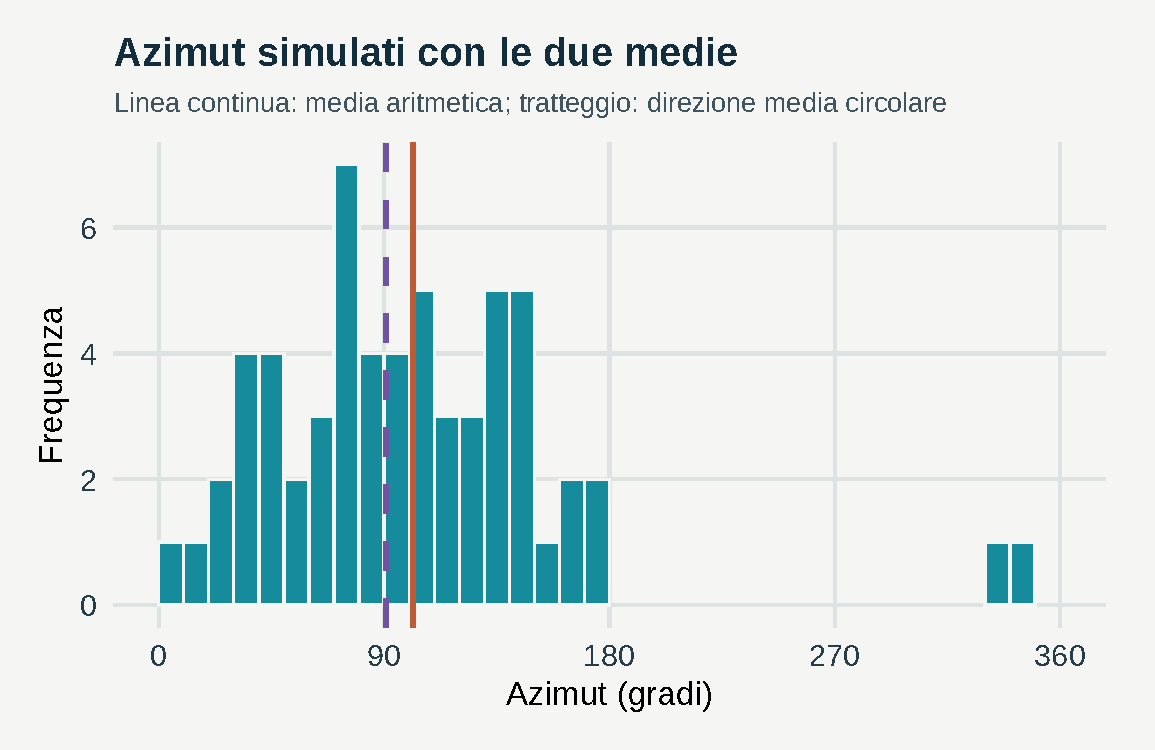
\includegraphics[width=\linewidth,height=6.0cm,keepaspectratio]{Esperimenti/m18-media-A.pdf}\par}
\PSmall{Direzione del generatore: 90 gradi; concentrazione 2. Seme: 17.}
}};
\node[anchor=north west,inner sep=0] at([xshift=10.85cm,yshift=-2.12cm]current page.north west){\Colonna{8.16cm}{\PLabel{Scenario A · simulazione}
\PBody{L’esperimento genera sessanta azimut da una distribuzione di von Mises con direzione $\mu$ e concentrazione $\kappa$. L’istogramma riporta la media aritmetica, linea continua, e la direzione media circolare, linea tratteggiata. Con $\mu=90^\circ$ le due medie distano 11 gradi.}
\par\smallskip{\centering\adjustbox{max width=.98\linewidth}{$\displaystyle \bar\theta=\operatorname{atan2}\Big(\frac1n\sum_i\sin\theta_i,\ \frac1n\sum_i\cos\theta_i\Big)$}\par\smallskip}
\PSmall{Lo scarto della media aritmetica cresce con la quota di misure che superano lo zero della scala.}
}};
\node[anchor=north east,inner sep=0] at([xshift=17.1cm,yshift=-12.04cm]current page.north west){\fontsize{7.7}{9}\selectfont \href{https://marzione00.github.io/Lab_Geo/\#laboratorio/m18-media}{\color{Classical}\bfseries Apri il laboratorio · m18-media}};
\end{tikzpicture}\end{frame}

\begin{frame}[plain]\hypertarget{slide9}{}
\bookmark[level=1,page=9]{Confronto | Media aritmetica e direzione media}
\begin{tikzpicture}[remember picture,overlay]
\PilotChrome{Confronto | Media aritmetica e direzione media}{ANGOLI E DIREZIONI MEDIE}{9}{La direzione media non cambia se si sposta l’origine della scala; la media aritmetica sì.}
\node[anchor=north west,inner sep=0] at([xshift=.96cm,yshift=-2.12cm]current page.north west){\Colonna{9.40cm}{{\centering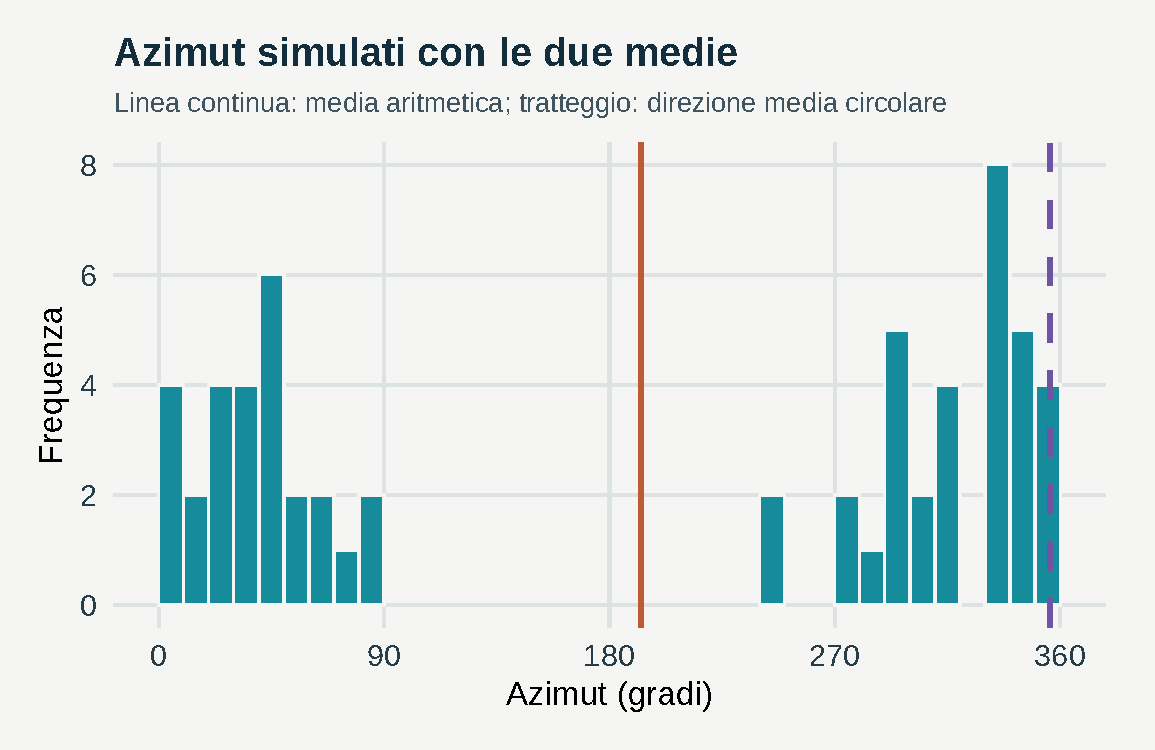
\includegraphics[width=\linewidth,height=5.6cm,keepaspectratio]{Esperimenti/m18-media-B.pdf}\par}
\PSmall{Direzione del generatore: 90 $\to$ 355 gradi. Tutti gli altri parametri e il seme sono fissi.}
}};
\node[anchor=north west,inner sep=0] at([xshift=10.85cm,yshift=-2.12cm]current page.north west){\Colonna{8.16cm}{\PLabel{Confronto fra gli scenari}
{\fontsize{10.2}{12.8}\selectfont\begin{tabular}{@{}>{\raggedright\arraybackslash}p{0.48\linewidth}@{\hspace{.13cm}}>{\raggedright\arraybackslash}p{0.224\linewidth}@{\hspace{.13cm}}>{\raggedright\arraybackslash}p{0.224\linewidth}@{}}\toprule Grandezza & A & B\\[2.3pt]
\midrule 
Direzione del generatore & 90 & 355\\[2.3pt]
Media aritmetica & 102 & 193\\[2.3pt]
Direzione media circolare & 90{,}9 & 356\\[2.3pt]
Scarto della media aritmetica & 11{,}7 & 162\\[2.3pt]
$\bar R$ & 0{,}697 & 0{,}697\\[2.3pt]
\bottomrule\end{tabular}\par}
\vspace{.25cm}\PBody{Con lo stesso seme i due scenari hanno le stesse direzioni ruotate di 265 gradi: $\bar R$ e lo scarto della direzione media restano uguali, lo scarto della media aritmetica sale a 162 gradi.}
}};
\node[anchor=north east,inner sep=0] at([xshift=17.1cm,yshift=-12.04cm]current page.north west){\fontsize{7.7}{9}\selectfont \href{https://marzione00.github.io/Lab_Geo/\#laboratorio/m18-media}{\color{Classical}\bfseries Apri il laboratorio · m18-media}};
\end{tikzpicture}\end{frame}

\begin{frame}[plain]\hypertarget{slide10}{}
\bookmark[level=0,page=10]{La distribuzione di von Mises}
\bookmark[level=1,page=10]{Un modello per direzioni concentrate}
\begin{tikzpicture}[remember picture,overlay]
\PilotChrome{Un modello per direzioni concentrate}{LA DISTRIBUZIONE DI VON MISES}{10}{La von Mises ha lo stesso ruolo della normale per i dati circolari: due parametri, $\mu$ e $\kappa$.}
\node[anchor=north west,inner sep=0] at([xshift=.96cm,yshift=-2.12cm]current page.north west){\Colonna{9.40cm}{{\centering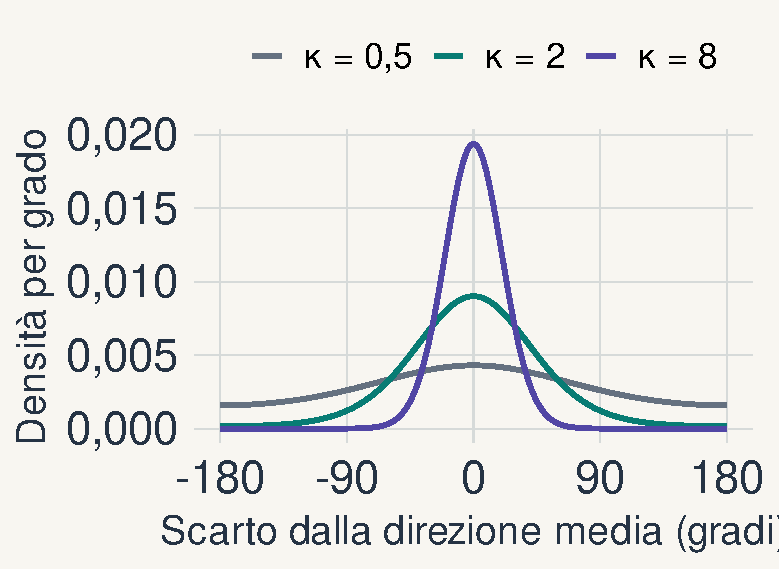
\includegraphics[width=\linewidth,height=6.15cm,keepaspectratio]{Figure/F02.pdf}\par}
\PSmall{Densità di von Mises per tre valori della concentrazione $\kappa$.}
}};
\node[anchor=north west,inner sep=0] at([xshift=10.85cm,yshift=-2.12cm]current page.north west){\Colonna{8.16cm}{\PBody{Richard von Mises introdusse nel 1918 una distribuzione sul cerchio con direzione media $\mu$ e concentrazione $\kappa$. Con $\kappa=0$ la distribuzione è uniforme; al crescere di $\kappa$ la densità si raccoglie attorno a $\mu$ e per valori grandi si avvicina a una normale con varianza $1/\kappa$. La costante $I_0$ è la funzione di Bessel modificata di ordine zero.}
\par\smallskip{\centering\adjustbox{max width=.98\linewidth}{$\displaystyle f(\theta)=\frac{e^{\kappa\cos(\theta-\mu)}}{2\pi I_0(\kappa)},\qquad 0\le\theta<2\pi$}\par\smallskip}
}};
\end{tikzpicture}\end{frame}

\begin{frame}[plain]\hypertarget{slide11}{}
\bookmark[level=1,page=11]{Stimare la concentrazione}
\begin{tikzpicture}[remember picture,overlay]
\PilotChrome{Stimare la concentrazione}{LA DISTRIBUZIONE DI VON MISES}{11}{La stima di massima verosimiglianza di $\kappa$ risolve $A_1(\kappa)=\bar R$.}
\node[anchor=north west,inner sep=0] at([xshift=.96cm,yshift=-2.12cm]current page.north west){\Colonna{9.40cm}{\PBody{La stima di massima verosimiglianza di $\mu$ è la direzione media; quella di $\kappa$ si ottiene uguagliando il rapporto fra due funzioni di Bessel alla lunghezza media risultante. Il codice risolve l’equazione per ogni stazione: S2 ha $\hat\kappa=10{,}84$, S6 soltanto 0,64. Per l’insieme delle misure $\hat\kappa$ vale 2,42.}
\par\smallskip{\centering\adjustbox{max width=.98\linewidth}{$\displaystyle A_1(\kappa)=\frac{I_1(\kappa)}{I_0(\kappa)}=\bar R$}\par\smallskip}
\PSmall{Con poche misure e $\bar R$ piccolo la stima di $\kappa$ è distorta verso l’alto.}
}};
\node[anchor=north west,inner sep=0] at([xshift=10.85cm,yshift=-2.12cm]current page.north west){\Colonna{8.16cm}{\begin{tcolorbox}[enhanced,arc=1.7mm,boxrule=.6pt,colback=white,colframe=Classical!60!Navy,colbacktitle=Navy,coltitle=white,fonttitle=\bfseries\small,title={R · calcolo riproducibile},left=1.7mm,right=1.3mm,top=1.1mm,bottom=1.1mm,before skip=1mm,after skip=1.0mm]\lstinputlisting[style=GeoR,language=R]{Codice/capitolo-03.R}\end{tcolorbox}
\PLabel{Risultato in R}
\begin{tcolorbox}[colback=GeoTint,colframe=Rule,boxrule=.5pt,arc=1.4mm,left=2mm,right=1mm,top=1mm,bottom=1mm]{\fontsize{8.6}{11.4}\selectfont\ttfamily \mbox{\ \ \ S1\ \ \ \ S2\ \ \ \ S3\ \ \ \ S4\ \ \ \ S5\ \ \ \ S6}\\\mbox{\ 3.92\ 10.84\ \ 3.30\ \ 6.02\ \ 3.18\ \ 0.64}}\end{tcolorbox}}};
\end{tikzpicture}\end{frame}

\begin{frame}[plain]\hypertarget{slide12}{}
\bookmark[level=1,page=12]{Le direzioni di S6 hanno una direzione preferenziale?}
\begin{tikzpicture}[remember picture,overlay]
\PilotChrome{{\fontsize{15.3}{19}\selectfont Le direzioni di S6 hanno una direzione preferenziale?}}{LA DISTRIBUZIONE DI VON MISES}{12}{Il test di Rayleigh confronta $\bar R$ con i valori attesi da direzioni uniformi.}
\node[anchor=north west,inner sep=0] at([xshift=.96cm,yshift=-2.12cm]current page.north west){\Colonna{9.40cm}{\PLabel{Domanda}
\PBody{In S1 venti lamine hanno $\bar R=0{,}86$, in S6 venti lamine hanno $\bar R=0{,}31$. Con venti misure, quale valore di $\bar R$ potrebbe nascere da direzioni distribuite in modo uniforme?}
\vspace{.35cm}\PLabel{Interpretazione}
\PBody{Per S1 la statistica $Z$ vale 14,8 e la probabilità di coda è inferiore a $10^{-4}$. Per S6 $Z=1{,}87$ e $p=0{,}155$: i dati di S6 sono compatibili con l’uniformità.}
}};
\node[anchor=north west,inner sep=0] at([xshift=10.85cm,yshift=-2.12cm]current page.north west){\Colonna{8.16cm}{\begin{tcolorbox}[enhanced,arc=1.7mm,boxrule=.6pt,colback=white,colframe=Classical!60!Navy,colbacktitle=Navy,coltitle=white,fonttitle=\bfseries\small,title={R · calcolo riproducibile},left=1.7mm,right=1.3mm,top=1.1mm,bottom=1.1mm,before skip=1mm,after skip=1.0mm]\lstinputlisting[style=GeoR,language=R]{Codice/capitolo-04.R}\end{tcolorbox}
\PLabel{Risultato in R}
\begin{tcolorbox}[colback=GeoTint,colframe=Rule,boxrule=.5pt,arc=1.4mm,left=2mm,right=1mm,top=1mm,bottom=1mm]{\fontsize{8.6}{11.4}\selectfont\ttfamily \mbox{\ \ \ \ \ \ \ S1\ \ \ \ \ \ S6}\\\mbox{n\ 20.0000\ 20.0000}\\\mbox{Z\ 14.8026\ \ 1.8658}\\\mbox{p\ \ 0.0000\ \ 0.1553}}\end{tcolorbox}}};
\end{tikzpicture}\end{frame}

\begin{frame}[plain]\hypertarget{slide13}{}
\bookmark[level=1,page=13]{Il test di Rayleigh nelle sei stazioni}
\begin{tikzpicture}[remember picture,overlay]
\PilotChrome{Il test di Rayleigh nelle sei stazioni}{LA DISTRIBUZIONE DI VON MISES}{13}{Con $n$ fissato, il test di Rayleigh equivale a confrontare $\bar R$ con una soglia.}
\node[anchor=north west,inner sep=0] at([xshift=.96cm,yshift=-2.12cm]current page.north west){\Colonna{9.40cm}{{\centering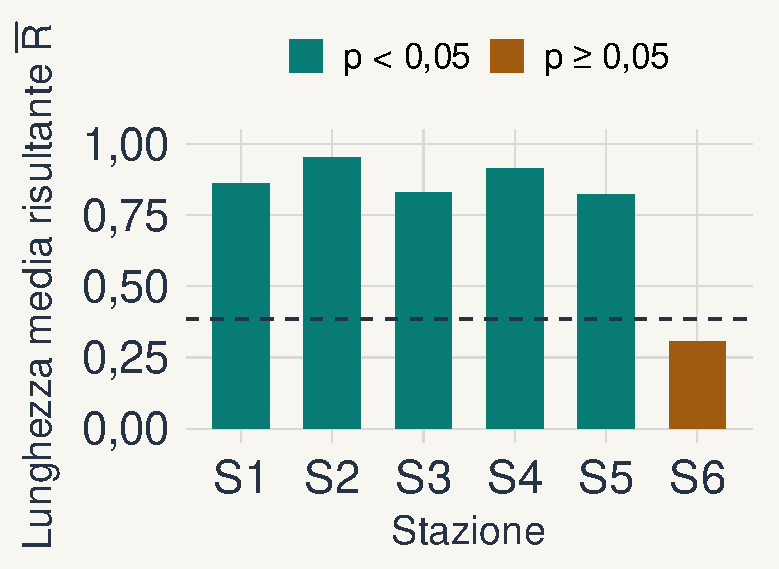
\includegraphics[width=\linewidth,height=6.15cm,keepaspectratio]{Figure/F03.pdf}\par}
\PSmall{Lunghezza media risultante per stazione; linea tratteggiata: valore critico 0,385 per $n=20$ al 5\%.}
}};
\node[anchor=north west,inner sep=0] at([xshift=10.85cm,yshift=-2.12cm]current page.north west){\Colonna{8.16cm}{\PBody{Lord Rayleigh studiò nel 1880 la somma di vibrazioni con fasi casuali, il problema da cui deriva il test. Sotto l’ipotesi di uniformità $2n\bar R^2$ segue approssimativamente una chi quadrato con due gradi di libertà; per campioni piccoli il codice della pagina precedente usa una correzione. Con venti misure la soglia al 5\% è $\bar R=0{,}385$: una simulazione di ventimila campioni uniformi dà 0,381.}
\par\smallskip{\centering\adjustbox{max width=.98\linewidth}{$\displaystyle Z=n\bar R^2,\qquad 2Z\approx\chi^2_2$}\par\smallskip}
}};
\end{tikzpicture}\end{frame}

\begin{frame}[plain]\hypertarget{slide14}{}
\bookmark[level=1,page=14]{Che cosa dice un test di uniformità}
\begin{tikzpicture}[remember picture,overlay]
\PilotChrome{Che cosa dice un test di uniformità}{LA DISTRIBUZIONE DI VON MISES}{14}{Un $p$ grande descrive dati compatibili con l’uniformità; la potenza dice quanto il test poteva vedere.}
\node[anchor=north west,inner sep=0] at([xshift=.96cm,yshift=-2.12cm]current page.north west){\Colonna{9.40cm}{\PLabel{Alternative unimodali}
\PBody{Il test di Rayleigh è costruito contro un’alternativa con una sola direzione preferenziale. Lamine oblique di ambiente tidale, con correnti di flusso e riflusso opposte, producono distribuzioni bimodali con modi a 180 gradi: la risultante si annulla e $\bar R$ resta piccolo anche se le direzioni sono concentrate. Per queste distribuzioni si usano gli angoli raddoppiati del capitolo successivo.}
}};
\node[anchor=north west,inner sep=0] at([xshift=10.85cm,yshift=-2.12cm]current page.north west){\Colonna{8.16cm}{\PLabel{Il caso di S6}
\PBody{Con venti misure il test ha potenza bassa per concentrazioni piccole: se le lamine di S6 seguissero una von Mises con $\kappa=0{,}64$, il test respingerebbe l’uniformità in circa quattro campioni su dieci. Il risultato di S6 indica direzioni molto disperse, e la direzione media di 309 gradi va riportata con la sua incertezza, oppure omessa.}
\PSmall{La potenza è la probabilità di respingere l’uniformità quando i dati hanno una direzione preferenziale.}
}};
\end{tikzpicture}\end{frame}

\begin{frame}[plain]\hypertarget{slide15}{}
\bookmark[level=1,page=15]{Potenza del test di Rayleigh}
\begin{tikzpicture}[remember picture,overlay]
\PilotChrome{Potenza del test di Rayleigh}{LA DISTRIBUZIONE DI VON MISES}{15}{Stimare con una simulazione la probabilità che il test riconosca una direzione preferenziale.}
\node[anchor=north west,inner sep=0] at([xshift=.96cm,yshift=-2.12cm]current page.north west){\Colonna{9.40cm}{{\centering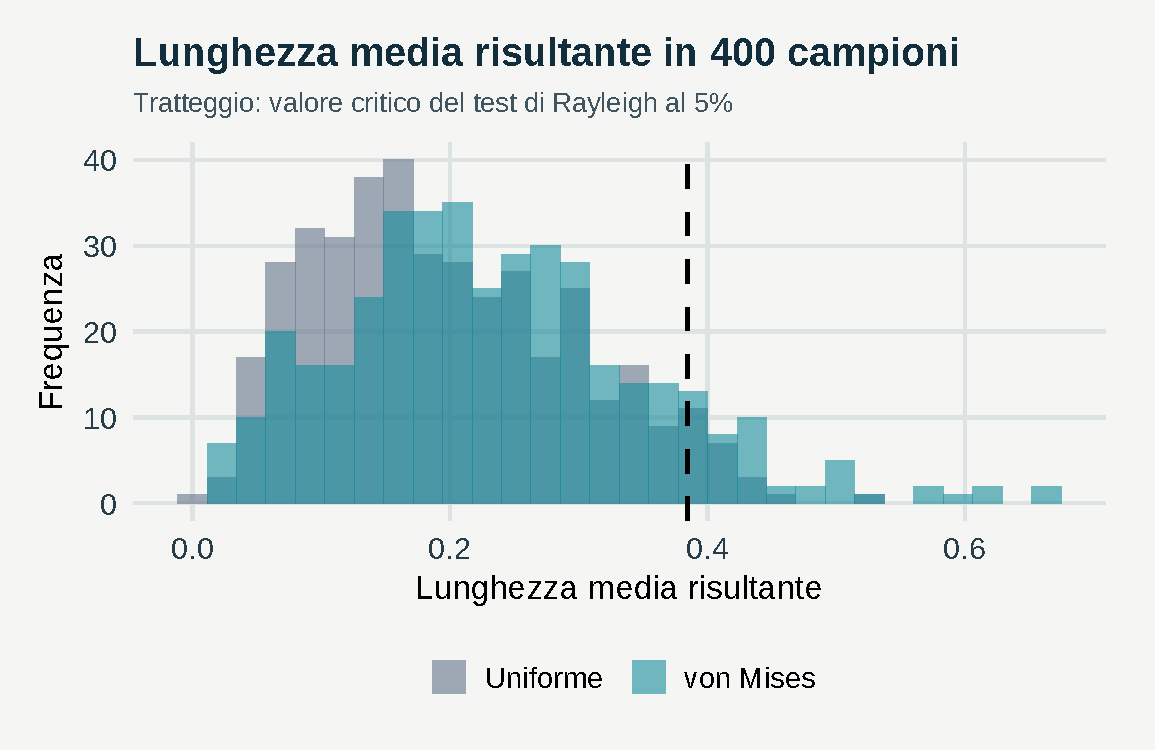
\includegraphics[width=\linewidth,height=6.0cm,keepaspectratio]{Esperimenti/m18-rayleigh-A.pdf}\par}
\PSmall{Concentrazione 0,3; venti misure; quattrocento campioni per ipotesi. Seme: 17.}
}};
\node[anchor=north west,inner sep=0] at([xshift=10.85cm,yshift=-2.12cm]current page.north west){\Colonna{8.16cm}{\PLabel{Scenario A · simulazione}
\PBody{L’esperimento simula quattrocento campioni da una von Mises e quattrocento da una distribuzione uniforme, con lo stesso $n$. L’istogramma confronta le due distribuzioni di $\bar R$ con il valore critico; la potenza è la quota di campioni von Mises con $p<0{,}05$.}
\par\smallskip{\centering\adjustbox{max width=.98\linewidth}{$\displaystyle \text{potenza}=P\big(p<0{,}05\mid\kappa,n\big)$}\par\smallskip}
\PSmall{La quota di rifiuti con dati uniformi controlla il livello del test, atteso al 5\%.}
}};
\node[anchor=north east,inner sep=0] at([xshift=17.1cm,yshift=-12.04cm]current page.north west){\fontsize{7.7}{9}\selectfont \href{https://marzione00.github.io/Lab_Geo/\#laboratorio/m18-rayleigh}{\color{Classical}\bfseries Apri il laboratorio · m18-rayleigh}};
\end{tikzpicture}\end{frame}

\begin{frame}[plain]\hypertarget{slide16}{}
\bookmark[level=1,page=16]{Confronto | Potenza del test di Rayleigh}
\begin{tikzpicture}[remember picture,overlay]
\PilotChrome{Confronto | Potenza del test di Rayleigh}{LA DISTRIBUZIONE DI VON MISES}{16}{Con venti misure il test riconosce una direzione preferenziale soltanto se la concentrazione è sufficiente.}
\node[anchor=north west,inner sep=0] at([xshift=.96cm,yshift=-2.12cm]current page.north west){\Colonna{9.40cm}{{\centering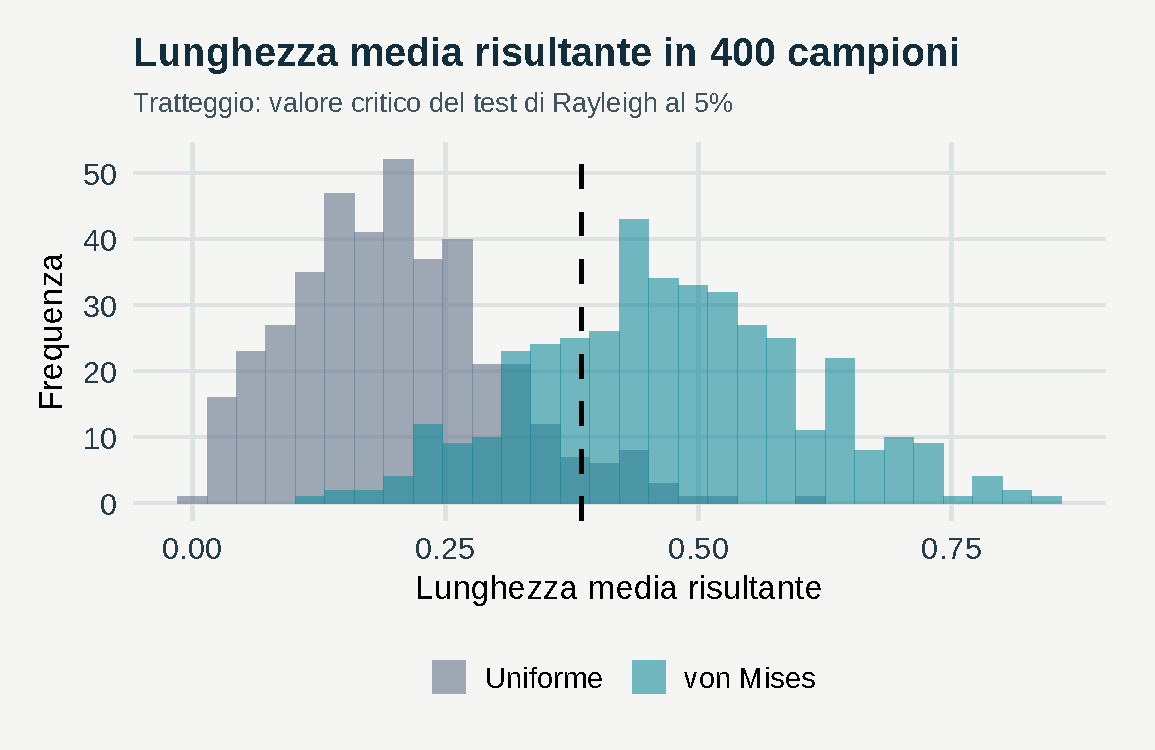
\includegraphics[width=\linewidth,height=5.6cm,keepaspectratio]{Esperimenti/m18-rayleigh-B.pdf}\par}
\PSmall{Concentrazione: 0,3 $\to$ 1. Tutti gli altri parametri e il seme sono fissi.}
}};
\node[anchor=north west,inner sep=0] at([xshift=10.85cm,yshift=-2.12cm]current page.north west){\Colonna{8.16cm}{\PLabel{Confronto fra gli scenari}
{\fontsize{10.2}{12.8}\selectfont\begin{tabular}{@{}>{\raggedright\arraybackslash}p{0.48\linewidth}@{\hspace{.13cm}}>{\raggedright\arraybackslash}p{0.224\linewidth}@{\hspace{.13cm}}>{\raggedright\arraybackslash}p{0.224\linewidth}@{}}\toprule Grandezza & A & B\\[2.3pt]
\midrule 
Potenza stimata & 0{,}113 & 0{,}748\\[2.3pt]
Rifiuti con dati uniformi & 0{,}045 & 0{,}0525\\[2.3pt]
Valore critico di $\bar R$ & 0{,}385 & 0{,}385\\[2.3pt]
$\bar R$ medio, von Mises & 0{,}235 & 0{,}471\\[2.3pt]
\bottomrule\end{tabular}\par}
\vspace{.25cm}\PBody{Con $\kappa=0{,}3$ la potenza è 0,113, poco sopra il livello; con $\kappa=1$ sale a 0,748. In entrambi gli scenari la quota di rifiuti con dati uniformi resta vicina a 0,05.}
}};
\node[anchor=north east,inner sep=0] at([xshift=17.1cm,yshift=-12.04cm]current page.north west){\fontsize{7.7}{9}\selectfont \href{https://marzione00.github.io/Lab_Geo/\#laboratorio/m18-rayleigh}{\color{Classical}\bfseries Apri il laboratorio · m18-rayleigh}};
\end{tikzpicture}\end{frame}

\begin{frame}[plain]\hypertarget{slide17}{}
\bookmark[level=0,page=17]{Dati assiali}
\bookmark[level=1,page=17]{Una linea non ha verso}
\begin{tikzpicture}[remember picture,overlay]
\PilotChrome{Una linea non ha verso}{DATI ASSIALI}{17}{Per dati assiali si raddoppiano gli angoli, si calcola la media e si divide per due.}
\node[anchor=north west,inner sep=0] at([xshift=.96cm,yshift=-2.12cm]current page.north west){\Colonna{9.40cm}{{\centering\resizebox{0.94\linewidth}{!}{\begin{tikzpicture}[x=1cm,y=1cm,every node/.append style={anchor=center,inner sep=.3333em}]
\begin{scope}
\draw[Rule,line width=.7pt] (0,0) circle(1.8);
\node[pNote] at(0,2.08){N};
\draw[GeoA,line width=1.3pt] ({1.8*sin(220)},{1.8*cos(220)})--({1.8*sin(40)},{1.8*cos(40)});
\fill[GeoA] ({1.8*sin(40)},{1.8*cos(40)}) circle(2.2pt) node[pLabel,anchor=south west]{$40^\circ$};
\fill[GeoA] ({1.8*sin(220)},{1.8*cos(220)}) circle(2.2pt) node[pLabel,anchor=north east]{$220^\circ$};
\node[pNote,text width=3.6cm] at(0,-2.55){Una linea, due estremità:\\$\theta$ e $\theta+180^\circ$.};
\end{scope}
\draw[pEdge] (2.2,0)--node[pLabel,above]{$\times 2$}(3.1,0);
\begin{scope}[xshift=5.3cm]
\draw[Rule,line width=.7pt] (0,0) circle(1.8);
\node[pNote] at(0,2.08){N};
\draw[-{Latex[length=2.4mm]},Classical,line width=1.3pt] (0,0)--({1.8*sin(80)},{1.8*cos(80)});
\fill[Classical] ({1.8*sin(80)},{1.8*cos(80)}) circle(2.2pt) node[pLabel,anchor=south,text=Classical,yshift=1mm]{$80^\circ$};
\node[pNote,text width=3.8cm] at(0,-2.55){$2\cdot 40^\circ=80^\circ$, $2\cdot 220^\circ=440^\circ\equiv 80^\circ$.\\L’asse è metà della direzione media.};
\end{scope}
\end{tikzpicture}
}\par}
\PSmall{La traccia di una frattura e il suo angolo raddoppiato.}
}};
\node[anchor=north west,inner sep=0] at([xshift=10.85cm,yshift=-2.12cm]current page.north west){\Colonna{8.16cm}{\PBody{La traccia di una frattura, un asse di piega o l’allungamento di un ciottolo sono linee: 40 e 220 gradi descrivono lo stesso oggetto. Raddoppiando gli angoli le due estremità coincidono, e i metodi per direzioni si applicano agli angoli $2\theta_i$. L’asse medio è metà della loro direzione media, fra 0 e 180 gradi.}
\par\smallskip{\centering\adjustbox{max width=.98\linewidth}{$\displaystyle \bar\theta_{\mathrm{asse}}=\tfrac12\operatorname{atan2}\big(\bar S_2,\bar C_2\big)$}\par\smallskip}
\PSmall{$\bar C_2$ e $\bar S_2$ sono le medie di $\cos2\theta_i$ e $\sin2\theta_i$.}
}};
\end{tikzpicture}\end{frame}

\begin{frame}[plain]\hypertarget{slide18}{}
\bookmark[level=1,page=18]{La famiglia J1 prima e dopo il raddoppio}
\begin{tikzpicture}[remember picture,overlay]
\PilotChrome{La famiglia J1 prima e dopo il raddoppio}{DATI ASSIALI}{18}{Un $\bar R$ vicino a zero può nascere da estremità registrate a caso.}
\node[anchor=north west,inner sep=0] at([xshift=.96cm,yshift=-2.12cm]current page.north west){\Colonna{9.40cm}{\PBody{Le settanta fratture della famiglia J1 sono annotate con l’una o l’altra estremità. Gli angoli registrati hanno $\bar R=0{,}036$, un valore che suggerirebbe direzioni uniformi. Gli angoli raddoppiati hanno $\bar R_2=0{,}930$ e l’asse medio è 42,6 gradi: la famiglia è fortemente orientata.}
\par\smallskip{\centering\adjustbox{max width=.98\linewidth}{$\displaystyle \bar R_2=\Big|\frac1n\sum_i\big(\cos2\theta_i,\ \sin2\theta_i\big)\Big|$}\par\smallskip}
}};
\node[anchor=north west,inner sep=0] at([xshift=10.85cm,yshift=-2.12cm]current page.north west){\Colonna{8.16cm}{\begin{tcolorbox}[enhanced,arc=1.7mm,boxrule=.6pt,colback=white,colframe=Classical!60!Navy,colbacktitle=Navy,coltitle=white,fonttitle=\bfseries\small,title={R · calcolo riproducibile},left=1.7mm,right=1.3mm,top=1.1mm,bottom=1.1mm,before skip=1mm,after skip=1.0mm]\lstinputlisting[style=GeoR,language=R]{Codice/capitolo-05.R}\end{tcolorbox}
\PLabel{Risultato in R}
\begin{tcolorbox}[colback=GeoTint,colframe=Rule,boxrule=.5pt,arc=1.4mm,left=2mm,right=1mm,top=1mm,bottom=1mm]{\fontsize{8.6}{11.4}\selectfont\ttfamily \mbox{\ \ \ \ \ R\ \ \ \ \ R2\ \ \ asse}\\\mbox{\ 0.036\ \ 0.930\ 42.597}}\end{tcolorbox}}};
\end{tikzpicture}\end{frame}

\begin{frame}[plain]\hypertarget{slide19}{}
\bookmark[level=1,page=19]{Due famiglie di fratture}
\begin{tikzpicture}[remember picture,overlay]
\PilotChrome{Due famiglie di fratture}{DATI ASSIALI}{19}{Una rosa assiale riporta ogni misura alle due estremità della linea.}
\node[anchor=north west,inner sep=0] at([xshift=.96cm,yshift=-2.12cm]current page.north west){\Colonna{9.40cm}{{\centering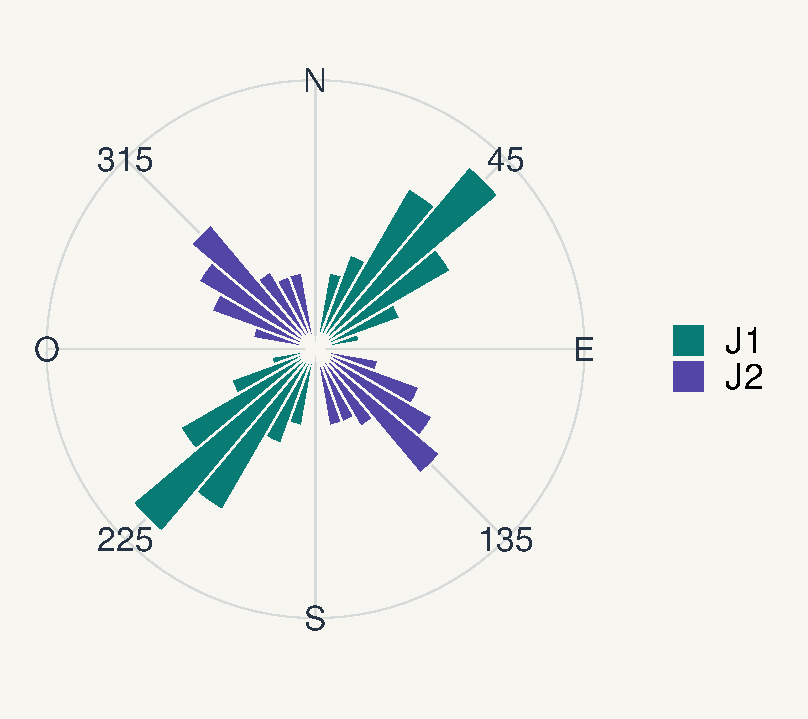
\includegraphics[width=\linewidth,height=6.15cm,keepaspectratio]{Figure/F04.pdf}\par}
\PSmall{Rosa assiale a settori di uguale area delle 110 fratture, in classi di 10 gradi, per famiglia.}
}};
\node[anchor=north west,inner sep=0] at([xshift=10.85cm,yshift=-2.12cm]current page.north west){\Colonna{8.16cm}{\PBody{La rosa mostra due famiglie. J1, settanta misure, ha asse medio 42,6 gradi; J2, quaranta misure, ha asse 132,0 gradi e $\bar R_2=0{,}871$. Gli assi delle due famiglie formano un angolo di 89,4 gradi. La rosa è simmetrica per costruzione, perché ogni linea compare due volte.}
\PSmall{L’attribuzione alle famiglie proviene dal rilievo di campagna, per esempio dai rapporti di intersezione.}
}};
\end{tikzpicture}\end{frame}

\begin{frame}[plain]\hypertarget{slide20}{}
\bookmark[level=1,page=20]{Riassumere prima di separare le famiglie}
\begin{tikzpicture}[remember picture,overlay]
\PilotChrome{Riassumere prima di separare le famiglie}{DATI ASSIALI}{20}{Due famiglie ortogonali diventano opposte negli angoli raddoppiati.}
\node[anchor=north west,inner sep=0] at([xshift=.96cm,yshift=-2.12cm]current page.north west){\Colonna{9.40cm}{\PLabel{Famiglie ortogonali}
\PBody{Il raddoppio trasforma una differenza di 90 gradi fra assi in una differenza di 180 gradi fra angoli raddoppiati. Le due famiglie del caso, prese insieme, hanno $\bar R_2=0{,}275$ e un asse medio di 43,3 gradi: il valore descrive J1, la famiglia più numerosa, e la concentrazione risulta molto più bassa di quella di ciascuna famiglia.}
\par\smallskip{\centering\adjustbox{max width=.98\linewidth}{$\displaystyle 2(\theta+90^\circ)=2\theta+180^\circ$}\par\smallskip}
}};
\node[anchor=north west,inner sep=0] at([xshift=10.85cm,yshift=-2.12cm]current page.north west){\Colonna{8.16cm}{\PLabel{Separare prima di riassumere}
\PBody{Un asse medio e una concentrazione hanno senso per una distribuzione unimodale. Con più famiglie si riassume ciascuna dopo averle separate con criteri di campagna o con un modello a miscela di distribuzioni di von Mises sugli angoli raddoppiati. La rosa assiale è il primo controllo della forma della distribuzione.}
\PSmall{Le stesse considerazioni valgono per assi di pieghe, lineazioni e orientazioni di clasti.}
}};
\end{tikzpicture}\end{frame}

\begin{frame}[plain]\hypertarget{slide21}{}
\bookmark[level=1,page=21]{Angoli raddoppiati e famiglie di fratture}
\begin{tikzpicture}[remember picture,overlay]
\PilotChrome{Angoli raddoppiati e famiglie di fratture}{DATI ASSIALI}{21}{Osservare il raddoppio degli angoli con una famiglia e con due famiglie.}
\node[anchor=north west,inner sep=0] at([xshift=.96cm,yshift=-2.12cm]current page.north west){\Colonna{9.40cm}{{\centering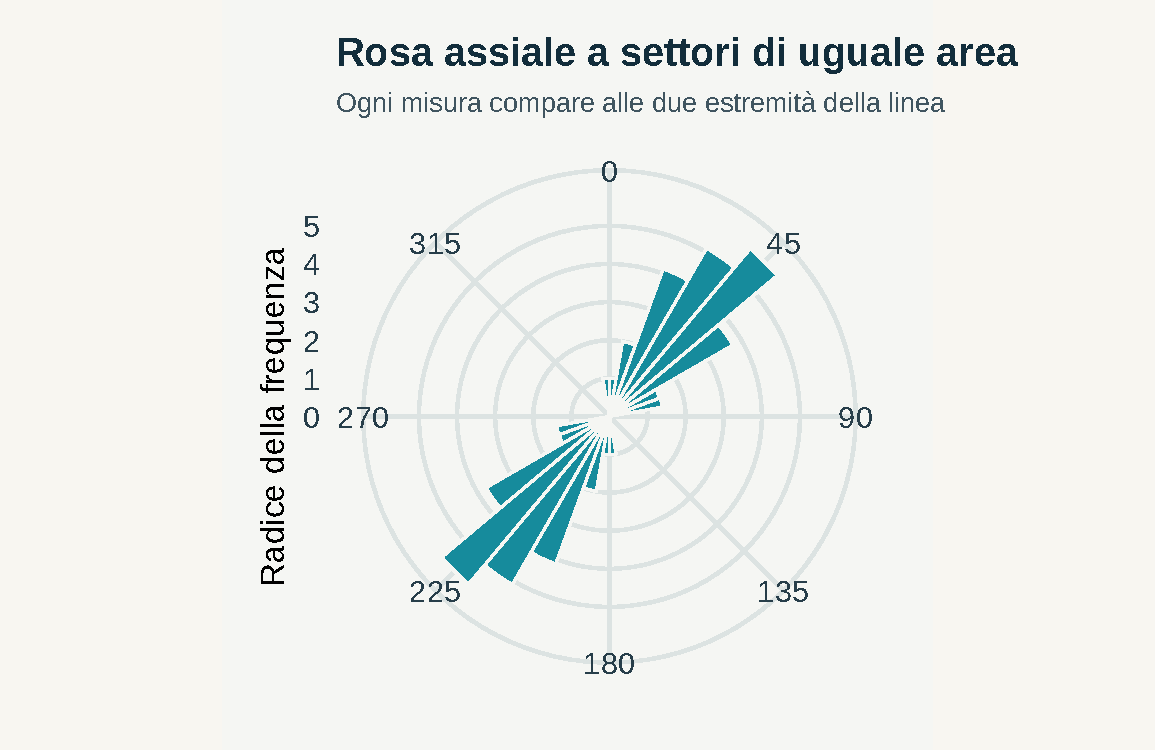
\includegraphics[width=\linewidth,height=6.0cm,keepaspectratio]{Esperimenti/m18-assiali-A.pdf}\par}
\PSmall{Una famiglia a 40 gradi; concentrazione degli angoli raddoppiati 6. Seme: 17.}
}};
\node[anchor=north west,inner sep=0] at([xshift=10.85cm,yshift=-2.12cm]current page.north west){\Colonna{8.16cm}{\PLabel{Scenario A · simulazione}
\PBody{L’esperimento genera cento direzioni attorno a una famiglia a 40 gradi e registra ogni misura con un’estremità scelta a caso. Con un angolo fra le famiglie maggiore di zero, metà delle misure forma una seconda famiglia. La rosa assiale ha settori di uguale area.}
\par\smallskip{\centering\adjustbox{max width=.98\linewidth}{$\displaystyle \bar R_2=\Big|\frac1n\sum_k e^{2\mathrm{i}\theta_k}\Big|$}\par\smallskip}
\PSmall{La notazione $e^{\mathrm{i}\theta_k}$ indica il vettore unitario $(\cos\theta_k,\sin\theta_k)$.}
}};
\node[anchor=north east,inner sep=0] at([xshift=17.1cm,yshift=-12.04cm]current page.north west){\fontsize{7.7}{9}\selectfont \href{https://marzione00.github.io/Lab_Geo/\#laboratorio/m18-assiali}{\color{Classical}\bfseries Apri il laboratorio · m18-assiali}};
\end{tikzpicture}\end{frame}

\begin{frame}[plain]\hypertarget{slide22}{}
\bookmark[level=1,page=22]{Confronto | Angoli raddoppiati e famiglie}
\begin{tikzpicture}[remember picture,overlay]
\PilotChrome{Confronto | Angoli raddoppiati e famiglie}{DATI ASSIALI}{22}{Il raddoppio risolve l’ambiguità delle estremità; la multimodalità resta da trattare.}
\node[anchor=north west,inner sep=0] at([xshift=.96cm,yshift=-2.12cm]current page.north west){\Colonna{9.40cm}{{\centering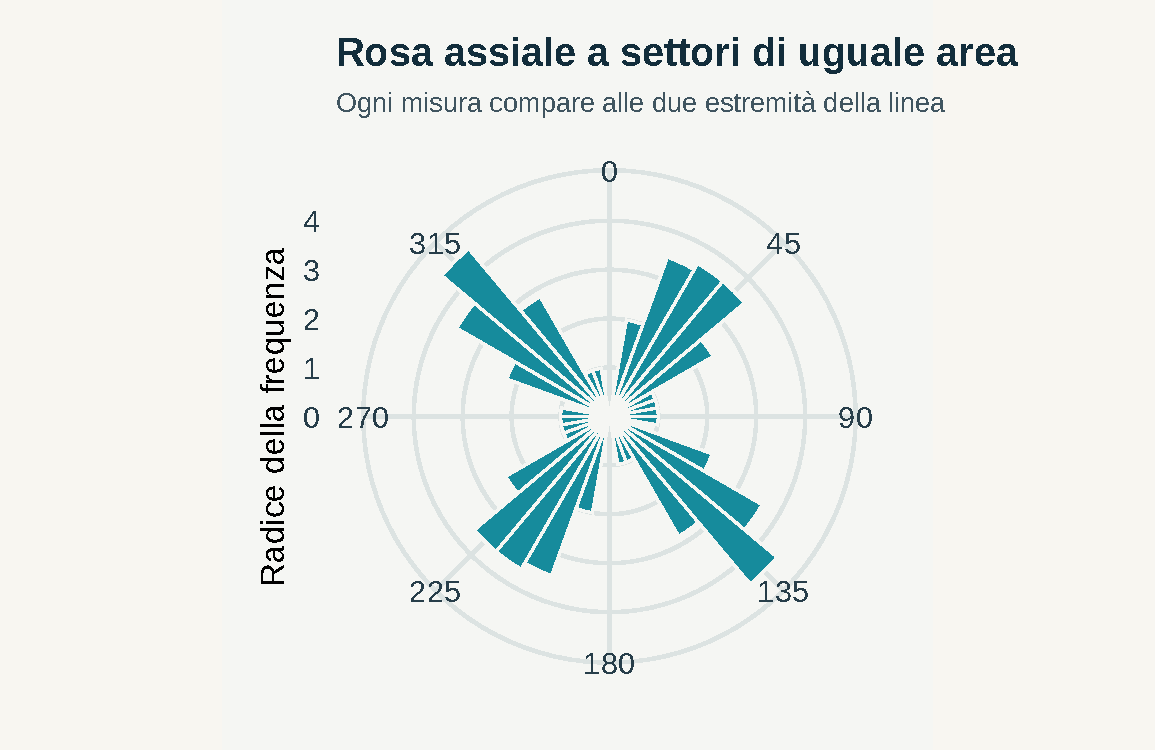
\includegraphics[width=\linewidth,height=5.6cm,keepaspectratio]{Esperimenti/m18-assiali-B.pdf}\par}
\PSmall{Angolo fra le famiglie: 0 $\to$ 90 gradi. Tutti gli altri parametri e il seme sono fissi.}
}};
\node[anchor=north west,inner sep=0] at([xshift=10.85cm,yshift=-2.12cm]current page.north west){\Colonna{8.16cm}{\PLabel{Confronto fra gli scenari}
{\fontsize{10.2}{12.8}\selectfont\begin{tabular}{@{}>{\raggedright\arraybackslash}p{0.48\linewidth}@{\hspace{.13cm}}>{\raggedright\arraybackslash}p{0.224\linewidth}@{\hspace{.13cm}}>{\raggedright\arraybackslash}p{0.224\linewidth}@{}}\toprule Grandezza & A & B\\[2.3pt]
\midrule 
$\bar R$ degli angoli registrati & 0{,}0726 & 0{,}0408\\[2.3pt]
$\bar R_2$ degli angoli raddoppiati & 0{,}901 & 0{,}0602\\[2.3pt]
Asse medio (gradi) & 39{,}3 & 173\\[2.3pt]
Angolo fra le famiglie & 0 & 90\\[2.3pt]
\bottomrule\end{tabular}\par}
\vspace{.25cm}\PBody{Con una famiglia $\bar R_2$ vale 0,901 e l’asse medio 39,3 gradi. Con due famiglie a 90 gradi $\bar R_2$ scende a 0,060 e l’asse medio di 173 gradi non descrive nessuna delle due.}
}};
\node[anchor=north east,inner sep=0] at([xshift=17.1cm,yshift=-12.04cm]current page.north west){\fontsize{7.7}{9}\selectfont \href{https://marzione00.github.io/Lab_Geo/\#laboratorio/m18-assiali}{\color{Classical}\bfseries Apri il laboratorio · m18-assiali}};
\end{tikzpicture}\end{frame}

\begin{frame}[plain]\hypertarget{slide23}{}
\bookmark[level=0,page=23]{Direzioni nello spazio}
\bookmark[level=1,page=23]{Coordinate e proiezione equivalente}
\begin{tikzpicture}[remember picture,overlay]
\PilotChrome{Coordinate e proiezione equivalente}{DIREZIONI NELLO SPAZIO}{23}{Nella proiezione equivalente aree uguali sulla sfera restano uguali nel piano.}
\node[anchor=north west,inner sep=0] at([xshift=.96cm,yshift=-2.12cm]current page.north west){\Colonna{9.40cm}{{\centering\resizebox{0.97\linewidth}{!}{\begin{tikzpicture}[x=1cm,y=1cm,every node/.append style={anchor=center,inner sep=.3333em}]
\draw[Rule,line width=.7pt] (-2.9,0)--(2.9,0);
\draw[Ink,line width=.8pt] (2.6,0) arc(0:-180:2.6);
\node[pNote,anchor=south west] at(-2.9,.05){orizzontale};
\fill[Ink] (0,0) circle(1.6pt) node[pNote,anchor=south]{$O$};
\coordinate (P) at ({2.6*cos(-35)},{2.6*sin(-35)});
\coordinate (B) at (0,-2.6);
\draw[-{Latex[length=2.4mm]},Classical,line width=1.2pt] (0,0)--(P) node[pLabel,anchor=west,text=Classical]{$P$};
\draw[Classical,line width=.6pt] (1.0,0) arc(0:-35:1.0);
\node[pLabel,text=Classical] at(1.25,-.32){$I$};
\draw[GeoB,line width=1.1pt] (B)--(P);
\draw[Muted,dashed] (0,0)--(B);
\draw[Muted,line width=.5pt] (0,-.7) arc(-90:-35:.7);
\node[pNote,text=Muted] at(.42,-1.02){$\theta$};
\fill[GeoB] (B) circle(1.8pt) node[pNote,anchor=north,text=GeoB]{$B$, verso il basso};
\node[pLabel,text=GeoB,anchor=west] at(1.25,-2.05){corda $\overline{BP}$};
\node[pNote,text width=7.2cm] at(0,-4.1){La proiezione equivalente porta $P$ a distanza dal centro pari alla corda $\overline{BP}=2\sin(\theta/2)$, con $\theta=90^\circ-I$. Dividendo per $\sqrt2$ l’orizzontale va sul cerchio di raggio 1.};
\end{tikzpicture}
}\par}
\PSmall{Sezione verticale dell’emisfero inferiore attraverso la direzione $OP$.}
}};
\node[anchor=north west,inner sep=0] at([xshift=10.85cm,yshift=-2.12cm]current page.north west){\Colonna{8.16cm}{\PBody{Una direzione nello spazio è data da un azimut, la declinazione $D$, e da un’inclinazione $I$ sotto l’orizzontale. I suoi coseni direttori sono le componenti verso nord, est e il basso. La proiezione equivalente di Lambert, il reticolo di Schmidt dei geologi, rappresenta l’emisfero inferiore conservando le aree: la densità dei punti nel piano rispecchia quella sulla sfera.}
\par\smallskip{\centering\adjustbox{max width=.98\linewidth}{$\displaystyle \mathbf x=(\cos I\cos D,\ \cos I\sin D,\ \sin I)$}\par\smallskip}
}};
\end{tikzpicture}\end{frame}

\begin{frame}[plain]\hypertarget{slide24}{}
\bookmark[level=1,page=24]{La media di Fisher delle quattordici colate}
\begin{tikzpicture}[remember picture,overlay]
\PilotChrome{La media di Fisher delle quattordici colate}{DIREZIONI NELLO SPAZIO}{24}{La direzione media nello spazio è quella della somma dei vettori unitari, come nel piano.}
\node[anchor=north west,inner sep=0] at([xshift=.96cm,yshift=-2.12cm]current page.north west){\Colonna{9.40cm}{\PBody{Ronald Fisher propose nel 1953 una distribuzione per direzioni disperse attorno a una media, discutendo dati paleomagnetici. La direzione media delle colate ha $D=344{,}8^\circ$ e $I=59{,}0^\circ$; la risultante misura 13,73 su 14 e la concentrazione stimata è $k=(N-1)/(N-R)=47{,}3$. Il cono di confidenza al 95\% ha semiangolo 5,84 gradi; l’approssimazione $140/\sqrt{kN}$ dà 5,44.}
\par\smallskip{\centering\adjustbox{max width=.98\linewidth}{$\displaystyle \cos\alpha_{95}=1-\frac{N-R}{R}\Big(20^{1/(N-1)}-1\Big)$}\par\smallskip}
}};
\node[anchor=north west,inner sep=0] at([xshift=10.85cm,yshift=-2.12cm]current page.north west){\Colonna{8.16cm}{\begin{tcolorbox}[enhanced,arc=1.7mm,boxrule=.6pt,colback=white,colframe=Classical!60!Navy,colbacktitle=Navy,coltitle=white,fonttitle=\bfseries\small,title={R · calcolo riproducibile},left=1.7mm,right=1.3mm,top=1.1mm,bottom=1.1mm,before skip=1mm,after skip=1.0mm]\lstinputlisting[style=GeoR,language=R]{Codice/capitolo-06.R}\end{tcolorbox}
\PLabel{Risultato in R}
\begin{tcolorbox}[colback=GeoTint,colframe=Rule,boxrule=.5pt,arc=1.4mm,left=2mm,right=1mm,top=1mm,bottom=1mm]{\fontsize{8.6}{11.4}\selectfont\ttfamily \mbox{\ \ \ \ \ D\ \ \ \ \ \ I\ \ \ \ \ \ R\ \ \ \ \ \ k\ \ \ \ a95}\\\mbox{344.83\ \ 58.97\ \ 13.73\ \ 47.34\ \ \ 5.84}}\end{tcolorbox}}};
\end{tikzpicture}\end{frame}

\begin{frame}[plain]\hypertarget{slide25}{}
\bookmark[level=1,page=25]{Le colate sul reticolo equivalente}
\begin{tikzpicture}[remember picture,overlay]
\PilotChrome{Le colate sul reticolo equivalente}{DIREZIONI NELLO SPAZIO}{25}{Il cono $\alpha_{95}$ è una regione di confidenza al 95\% per la direzione media, se il modello di Fisher è adeguato.}
\node[anchor=north west,inner sep=0] at([xshift=.96cm,yshift=-2.12cm]current page.north west){\Colonna{9.40cm}{{\centering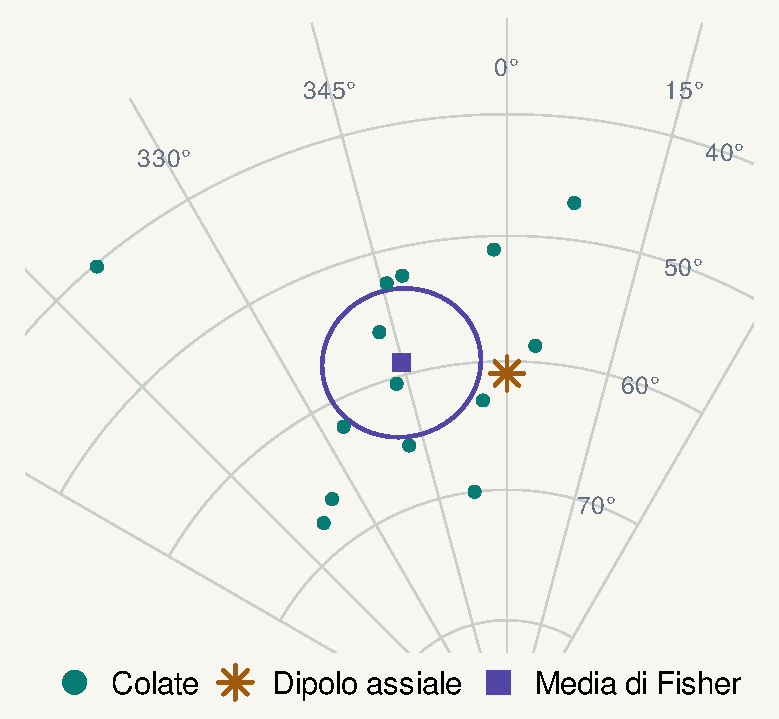
\includegraphics[width=\linewidth,height=6.15cm,keepaspectratio]{Figure/F05.pdf}\par}
\PSmall{Particolare della proiezione equivalente, emisfero inferiore, con linee di uguale declinazione e cerchi di uguale inclinazione.}
}};
\node[anchor=north west,inner sep=0] at([xshift=10.85cm,yshift=-2.12cm]current page.north west){\Colonna{8.16cm}{\PBody{I quattordici punti sono le direzioni delle colate; il quadrato è la media di Fisher e il cerchio il cono $\alpha_{95}$. L’asterisco è la direzione del campo di un dipolo assiale geocentrico alla latitudine del sito, 42 gradi nord: declinazione 0, inclinazione 60,96 gradi. L’asterisco cade fuori dal cono.}
\PSmall{Nel paleomagnetismo $N$ conta le colate, perché ogni colata registra un istante del campo.}
}};
\end{tikzpicture}\end{frame}

\begin{frame}[plain]\hypertarget{slide26}{}
\bookmark[level=1,page=26]{Il sito ha ruotato attorno a un asse verticale?}
\begin{tikzpicture}[remember picture,overlay]
\PilotChrome{Il sito ha ruotato attorno a un asse verticale?}{DIREZIONI NELLO SPAZIO}{26}{Per un dipolo assiale geocentrico l’inclinazione dipende soltanto dalla latitudine.}
\node[anchor=north west,inner sep=0] at([xshift=.96cm,yshift=-2.12cm]current page.north west){\Colonna{9.40cm}{\PLabel{Domanda}
\PBody{Per un dipolo assiale geocentrico $\tan I=2\tan\lambda$ e la declinazione è zero. La direzione media delle colate è compatibile con il campo atteso alla latitudine del sito?}
\vspace{.35cm}\PLabel{Interpretazione}
\PBody{L’inclinazione attesa è 60,96 gradi e la direzione attesa dista 7,83 gradi dalla media, più del raggio del cono. La declinazione di 344,8 gradi suggerisce una rotazione antioraria di circa 15 gradi, da confermare con altri siti.}
}};
\node[anchor=north west,inner sep=0] at([xshift=10.85cm,yshift=-2.12cm]current page.north west){\Colonna{8.16cm}{\begin{tcolorbox}[enhanced,arc=1.7mm,boxrule=.6pt,colback=white,colframe=Classical!60!Navy,colbacktitle=Navy,coltitle=white,fonttitle=\bfseries\small,title={R · calcolo riproducibile},left=1.7mm,right=1.3mm,top=1.1mm,bottom=1.1mm,before skip=1mm,after skip=1.0mm]\lstinputlisting[style=GeoR,language=R]{Codice/capitolo-07.R}\end{tcolorbox}
\PLabel{Risultato in R}
\begin{tcolorbox}[colback=GeoTint,colframe=Rule,boxrule=.5pt,arc=1.4mm,left=2mm,right=1mm,top=1mm,bottom=1mm]{\fontsize{8.6}{11.4}\selectfont\ttfamily \mbox{\ \ \ I\_gad\ distanza}\\\mbox{\ \ \ 60.96\ \ \ \ \ 7.83}}\end{tcolorbox}}};
\end{tikzpicture}\end{frame}

\begin{frame}[plain]\hypertarget{slide27}{}
\bookmark[level=1,page=27]{I poli degli strati descrivono una cintura}
\begin{tikzpicture}[remember picture,overlay]
\PilotChrome{I poli degli strati descrivono una cintura}{DIREZIONI NELLO SPAZIO}{27}{In una piega cilindrica i poli degli strati giacciono su un cerchio massimo normale all’asse.}
\node[anchor=north west,inner sep=0] at([xshift=.96cm,yshift=-2.12cm]current page.north west){\Colonna{9.40cm}{{\centering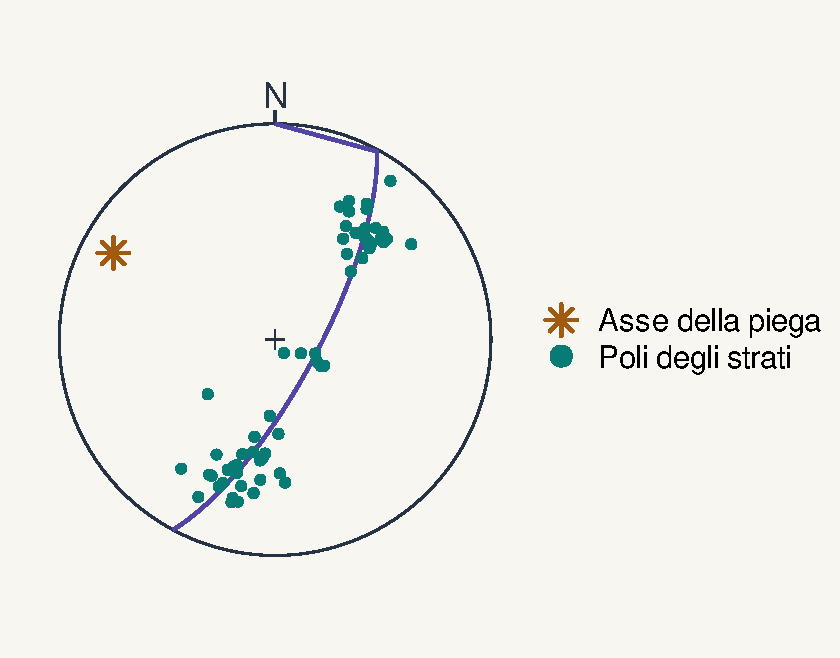
\includegraphics[width=\linewidth,height=6.15cm,keepaspectratio]{Figure/F06.pdf}\par}
\PSmall{Poli dei sessanta strati, cerchio massimo meglio adattato e asse della piega.}
}};
\node[anchor=north west,inner sep=0] at([xshift=10.85cm,yshift=-2.12cm]current page.north west){\Colonna{8.16cm}{\PBody{I poli della stratificazione si dispongono lungo un cerchio massimo: i due fianchi formano due gruppi e la cerniera li collega. La loro lunghezza media risultante, 0,64, rende la media di Fisher poco informativa. L’asse della piega è la direzione normale al cerchio massimo meglio adattato ai poli.}
\PSmall{I poli sono assi: il segno del vettore non conta, e il loro riassunto usa prodotti $\mathbf x\mathbf x^{\mathsf T}$.}
}};
\end{tikzpicture}\end{frame}

\begin{frame}[plain]\hypertarget{slide28}{}
\bookmark[level=1,page=28]{Il tensore di orientazione e l’asse della piega}
\begin{tikzpicture}[remember picture,overlay]
\PilotChrome{Il tensore di orientazione e l’asse della piega}{DIREZIONI NELLO SPAZIO}{28}{Autovalori del tensore di orientazione: forma della distribuzione; autovettori: direzioni principali.}
\node[anchor=north west,inner sep=0] at([xshift=.96cm,yshift=-2.12cm]current page.north west){\Colonna{9.40cm}{\PBody{Il tensore di orientazione è la media dei prodotti $\mathbf x_i\mathbf x_i^{\mathsf T}$ e tratta allo stesso modo un polo e il suo opposto. Gli autovalori valgono 0,564, 0,422 e 0,014: l’ultimo, quasi nullo, indica una cintura. L’autovettore corrispondente fornisce l’asse della piega, 298 gradi con immersione di 16 gradi. Nigel Woodcock propose nel 1977 il parametro $K$, qui 0,086: valori minori di 1 indicano cinture.}
\par\smallskip{\centering\adjustbox{max width=.98\linewidth}{$\displaystyle T=\frac1n\sum_i\mathbf x_i\mathbf x_i^{\mathsf T},\qquad K=\frac{\log(S_1/S_2)}{\log(S_2/S_3)}$}\par\smallskip}
}};
\node[anchor=north west,inner sep=0] at([xshift=10.85cm,yshift=-2.12cm]current page.north west){\Colonna{8.16cm}{\begin{tcolorbox}[enhanced,arc=1.7mm,boxrule=.6pt,colback=white,colframe=Classical!60!Navy,colbacktitle=Navy,coltitle=white,fonttitle=\bfseries\small,title={R · calcolo riproducibile},left=1.7mm,right=1.3mm,top=1.1mm,bottom=1.1mm,before skip=1mm,after skip=1.0mm]\lstinputlisting[style=GeoR,language=R]{Codice/capitolo-08.R}\end{tcolorbox}
\PLabel{Risultato in R}
\begin{tcolorbox}[colback=GeoTint,colframe=Rule,boxrule=.5pt,arc=1.4mm,left=2mm,right=1mm,top=1mm,bottom=1mm]{\fontsize{8.6}{11.4}\selectfont\ttfamily \mbox{\ \ \ \ \ S1\ \ \ \ \ \ S2\ \ \ \ \ \ S3\ \ \ trend\ \ plunge}\\\mbox{\ \ 0.564\ \ \ 0.422\ \ \ 0.014\ 298.205\ \ 16.097}}\end{tcolorbox}}};
\end{tikzpicture}\end{frame}

\begin{frame}[plain]\hypertarget{slide29}{}
\bookmark[level=1,page=29]{Cono di confidenza di Fisher}
\begin{tikzpicture}[remember picture,overlay]
\PilotChrome{Cono di confidenza di Fisher}{DIREZIONI NELLO SPAZIO}{29}{Osservare come il cono di confidenza si restringe al crescere del numero di direzioni.}
\node[anchor=north west,inner sep=0] at([xshift=.96cm,yshift=-2.12cm]current page.north west){\Colonna{9.40cm}{{\centering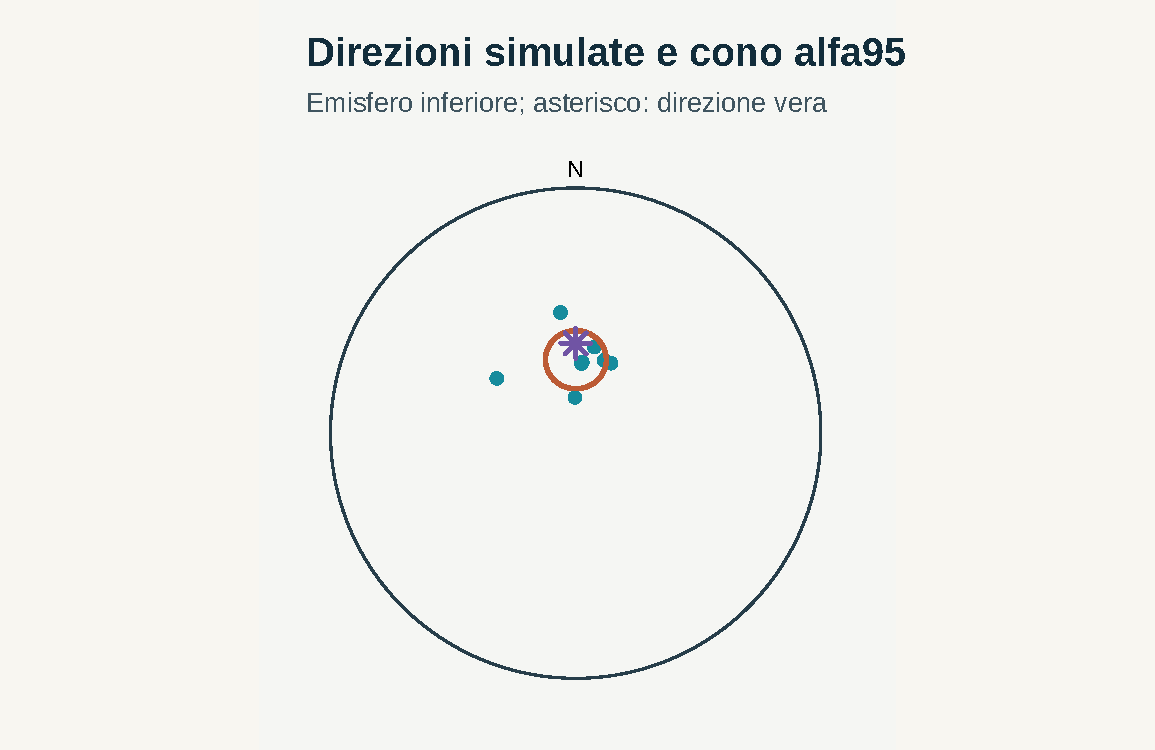
\includegraphics[width=\linewidth,height=6.0cm,keepaspectratio]{Esperimenti/m18-fisher-A.pdf}\par}
\PSmall{Otto direzioni; concentrazione 30. Seme: 17.}
}};
\node[anchor=north west,inner sep=0] at([xshift=10.85cm,yshift=-2.12cm]current page.north west){\Colonna{8.16cm}{\PLabel{Scenario A · simulazione}
\PBody{L’esperimento genera $N$ direzioni da una distribuzione di Fisher attorno a una direzione vera con declinazione 0 e inclinazione 60 gradi. Il grafico riporta le direzioni, il cono $\alpha_{95}$ attorno alla media stimata e la direzione vera.}
\par\smallskip{\centering\adjustbox{max width=.98\linewidth}{$\displaystyle \alpha_{95}\approx\frac{140^\circ}{\sqrt{kN}}$}\par\smallskip}
\PSmall{$k$ è stimato dai dati simulati; il valore del generatore è fissato dal controllo.}
}};
\node[anchor=north east,inner sep=0] at([xshift=17.1cm,yshift=-12.04cm]current page.north west){\fontsize{7.7}{9}\selectfont \href{https://marzione00.github.io/Lab_Geo/\#laboratorio/m18-fisher}{\color{Classical}\bfseries Apri il laboratorio · m18-fisher}};
\end{tikzpicture}\end{frame}

\begin{frame}[plain]\hypertarget{slide30}{}
\bookmark[level=1,page=30]{Confronto | Cono di confidenza di Fisher}
\begin{tikzpicture}[remember picture,overlay]
\PilotChrome{Confronto | Cono di confidenza di Fisher}{DIREZIONI NELLO SPAZIO}{30}{Il cono si restringe circa come $1/\sqrt N$; con poche direzioni l’approssimazione lo sottostima.}
\node[anchor=north west,inner sep=0] at([xshift=.96cm,yshift=-2.12cm]current page.north west){\Colonna{9.40cm}{{\centering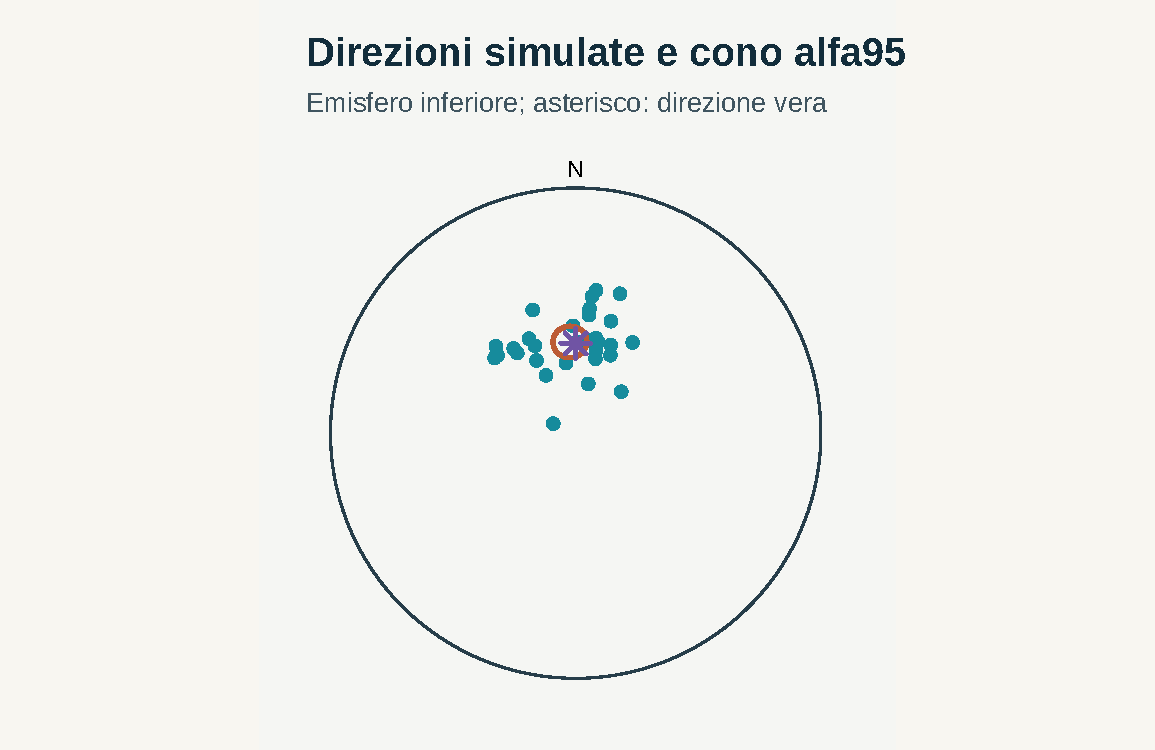
\includegraphics[width=\linewidth,height=5.6cm,keepaspectratio]{Esperimenti/m18-fisher-B.pdf}\par}
\PSmall{Numero di direzioni: 8 $\to$ 30. Tutti gli altri parametri e il seme sono fissi.}
}};
\node[anchor=north west,inner sep=0] at([xshift=10.85cm,yshift=-2.12cm]current page.north west){\Colonna{8.16cm}{\PLabel{Confronto fra gli scenari}
{\fontsize{10.2}{12.8}\selectfont\begin{tabular}{@{}>{\raggedright\arraybackslash}p{0.48\linewidth}@{\hspace{.13cm}}>{\raggedright\arraybackslash}p{0.224\linewidth}@{\hspace{.13cm}}>{\raggedright\arraybackslash}p{0.224\linewidth}@{}}\toprule Grandezza & A & B\\[2.3pt]
\midrule 
$\alpha_{95}$ (gradi) & 9{,}84 & 5{,}4\\[2.3pt]
$140/\sqrt{kN}$ (gradi) & 8{,}66 & 5{,}15\\[2.3pt]
$k$ stimato & 32{,}6 & 24{,}6\\[2.3pt]
Distanza dalla direzione vera & 5{,}45 & 1{,}92\\[2.3pt]
\bottomrule\end{tabular}\par}
\vspace{.25cm}\PBody{Con otto direzioni $\alpha_{95}$ vale 9,84 gradi e l’approssimazione 8,66; con trenta direzioni i due valori sono 5,40 e 5,15. In entrambi i casi la direzione vera cade dentro il cono.}
}};
\node[anchor=north east,inner sep=0] at([xshift=17.1cm,yshift=-12.04cm]current page.north west){\fontsize{7.7}{9}\selectfont \href{https://marzione00.github.io/Lab_Geo/\#laboratorio/m18-fisher}{\color{Classical}\bfseries Apri il laboratorio · m18-fisher}};
\end{tikzpicture}\end{frame}

\begin{frame}[plain]\hypertarget{slide31}{}
\bookmark[level=0,page=31]{Sintesi}
\bookmark[level=1,page=31]{Dal risultato alla relazione}
\begin{tikzpicture}[remember picture,overlay]
\PilotChrome{Dal risultato alla relazione}{SINTESI}{31}{Riporta direzione media, $\bar R$ o $k$, numero di misure e cono di confidenza.}
\node[anchor=north west,inner sep=0] at([xshift=.96cm,yshift=-2.12cm]current page.north west){\Colonna{9.40cm}{\PLabel{Domanda di partenza}
\PBody{Le paleocorrenti erano dirette verso 202,5 gradi?}
\PLabel{Risultato da discutere}
\PBody{Le paleocorrenti hanno direzione media di 352,4 gradi, verso nord: la media aritmetica di 202,5 gradi nasce dalla posizione dello zero della scala. Cinque stazioni hanno una direzione preferenziale netta; S6 è compatibile con l’uniformità. Le fratture formano due famiglie quasi ortogonali, le colate suggeriscono una rotazione antioraria di circa 15 gradi e la piega ha asse 298/16.}
}};
\node[anchor=north west,inner sep=0] at([xshift=10.85cm,yshift=-2.12cm]current page.north west){\Colonna{8.16cm}{\PLabel{Limiti della conclusione}
\PBody{I dati sono sintetici. Il test di Rayleigh e il cono di Fisher presuppongono misure indipendenti e distribuzioni unimodali e simmetriche; con venti misure per stazione la potenza è bassa per concentrazioni piccole, e una sola località paleomagnetica non basta a stabilire una rotazione.}
\vspace{.4cm}\href{https://marzione00.github.io/Lab_Geo/\#modulo-M18}{\color{Classical}\bfseries Torna agli esperimenti di Azimut}
}};
\end{tikzpicture}\end{frame}

\begin{frame}[plain]\hypertarget{slide32}{}
\bookmark[level=0,page=32]{Riferimenti}
\bookmark[level=1,page=32]{Fonti, dati e codice per riprodurre le figure}
\begin{tikzpicture}[remember picture,overlay]
\PilotChrome{Fonti, dati e codice per riprodurre le figure}{RIFERIMENTI}{32}{I risultati numerici si riferiscono ai dati e alle ipotesi dichiarate nel caso.}
\node[anchor=north west,inner sep=0] at([xshift=.96cm,yshift=-2.12cm]current page.north west){\Colonna{9.40cm}{\PLabel{Fonti}
{\fontsize{9.4}{12.2}\selectfont Lord Rayleigh, Philosophical Magazine 10(60), 73–78, 1880.\par R. A. Fisher, Proceedings of the Royal Society of London A 217, 295–305, 1953.\par J. R. Curray, Journal of Geology 64(2), 117–131, 1956.\par N. H. Woodcock, Geological Society of America Bulletin 88, 1231–1236, 1977.\par D. J. Best e N. I. Fisher, Applied Statistics 28(2), 152–157, 1979.\par W. Nemec, Sedimentary Geology 59, 149–152, 1988.\par R. F. Butler, Paleomagnetism: Magnetic Domains to Geologic Terranes, Blackwell, 1992.\par N. I. Fisher, Statistical Analysis of Circular Data, Cambridge University Press, 1993.\par K. V. Mardia e P. E. Jupp, Directional Statistics, Wiley, 2000.\par D. J. Sanderson e D. C. P. Peacock, Earth-Science Reviews 201, 103055, 2020.\par}
}};
\node[anchor=north west,inner sep=0] at([xshift=10.85cm,yshift=-2.12cm]current page.north west){\Colonna{8.16cm}{\PLabel{Dati e codice}
\PBody{Dati sintetici del corso (correnti\_v1.csv, fratture\_v1.csv, paleomag\_v1.csv, strati\_v1.csv), generati da R/genera\_dati.R. Codice contiene i frammenti delle pagine; R/M18\_figure.R ricostruisce figure e valori; Esperimenti contiene i programmi dei due scenari e Diagrammi i disegni TikZ.}
\vspace{.3cm}\href{https://marzione00.github.io/Lab_Geo/\#lezione-M18}{\color{Classical}\bfseries Apri le tappe di Azimut su GeoStat Lab}
}};
\end{tikzpicture}\end{frame}
\end{document}
